\documentclass[12pt]{ociamthesis}  % default square logo 
% \documentclass[12pt,beltcrest]{ociamthesis} % use old belt crest logo
%\documentclass[12pt,shieldcrest]{ociamthesis} % use older shield crest logo

%load any additional packages

% ---- START OF CUSTOM CONFIGURATION ----

\usepackage{amssymb} % unknown
\usepackage{array} % unknown
\usepackage{courier} % give courier font to listings and also \texttt{}
\usepackage{xcolor} % add colors to text using \textcolor{red}{<text>}
\usepackage{amsmath} % unknown
\usepackage{ulem} % unknown
\usepackage{hyperref} % ability to add links using \href{<link>}{<label>}, also ability to make the contents page clickable
\usepackage{listings} % ability to print code using \begin{lstlisting}
\usepackage{graphicx} % ability to add image
\usepackage{tablefootnote} % ability to use table footnotes in table using command \tablefootnotes
\usepackage{multirow} % ability to merge rows using \mergerow
\usepackage{makecell} % ability to have line breaks inside tables
\usepackage{imakeidx} % add an index for the document
\makeindex % add an index for the document
% configure hyperref, display the contents page as its usual black color
\hypersetup{ 
    colorlinks,
    citecolor=black,
    filecolor=black,
    linkcolor=black,
    urlcolor=black
}

% configure listings
\lstset{language=Python}
\lstset{basicstyle=\ttfamily,breaklines=true} %use courier as font, also make sure it skips to another line when the text is too long for one line

\setlength{\parindent}{0pt} % disable indent of first line of each paragraph
\graphicspath{ {./images/} } % configure graphicx

% ---- END OF CUSTOM CONFIGURATION ----

%input macros (i.e. write your own macros file called mymacros.tex 
%and uncomment the next line)
%\include{mymacros}

\title{Web \& Git Dictionary}   %note \\[1ex] is a line break in the title

\author{Oscar Mui }             %your name
\college{University College}  %your college

% \renewcommand{Notes for}{change the default text here if needed}
\degree{CompSoc Learn to Code } %\\[1ex] (in Python)     %the degree
\degreedate{Hilary 2023}         %the degree date

%end the preamble and start the document
\begin{document}

%this baselineskip gives sufficient line spacing for an examiner to easily
%markup the thesis with comments
\baselineskip=18pt plus1pt

%set the number of sectioning levels that get number and appear in the contents
\setcounter{secnumdepth}{3}
\setcounter{tocdepth}{3}


\maketitle                  % create a title page from the preamble info
\include{dedication}        % include a dedication.tex file
\include{acknowlegements}   % include an acknowledgements.tex file
\chapter*{Preface}

This piece of notes covers one way of building a \textbf{static} website. It facilitates my live teaching sessions or my Web \& Git YouTube series.
\vspace{6mm}

We use \textbf{Pug.js} (sometimes abbreviated to Pug in this piece of notes) instead of HTML, \textbf{less} instead of CSS. And used gulp to translate the files back to HTML and CSS. The generated HTML files can be directly opened by the browser. We also included \textbf{Bootstrap} to make our static website responsive.
\vspace{6mm}

At the same time, we will be learning how to use \textbf{Git} and \textbf{command line tools}.

\section{Prerequisites}

Basic coding experience (e.g. variables, loops) in any programming languages (e.g. C++, Python) is expected. Knowing basic HTML and CSS would be helpful, but not necessary. 
% I would contrast HTML with Pug.js and CSS with less throughout the notes, if you have not learned HTML and CSS you could skip those sessions.

\section{Way to read the notes}

This piece of notes aims to fill the gaps of the online resources, and also acts as the bridge between different components of the project. It will not include every detail that you need to know, but I would try to include different online resources (documentations and YouTube tutorials) required in the form of hyperlinks along the way.
\vspace{6mm}

Hands on practice is also super important in programming, instead of revising this piece of notes over and over again, you will probably learn more if you make more websites on your own. :)
\vspace{6mm}

We start with installing the tools you need for this project. It is probably a bit complicated for most of you, but I reassure you that it is worth the time. It also tells you some basic tips to use the project. In order for you to have hands on experience with coding as soon as possible, \cref{sec:pug1} introduces the Pug.js syntax allowing you to edit the content of the web page. Then we go back to some boring\footnote{I guess the command line interface is not colourful is what makes it boring?} details in chapters 3-6. Then we go back to talk about styling in chapters 7-8. Finally, we will learn how to use variables in Pug.js in \cref{sec:pug2}. And we conclude by miscellaneous bits in \cref{sec:misc}.
\vspace{6mm}

I marked the less essential sections with \textit{Advanced} or \textit{Of less importance}. The whole of \cref{sec:git2} and \cref{sec:pug2} are labelled with \textit{Advanced}, while the whole of \cref{sec:misc} is labelled with \textit{Of less importance}. You can read the sections without the markings first, then those with \textit{Advanced}, then those with \textit{Of less importance}.

\section{Why?}

Why are we learning how to make a website? Why this particular framework? Why are we learning Git and command line tools at the same time?

I decided to delay answering these questions until the last chapter \cref{sec:rationale}, as it is easier to explain after you have learnt all the knowledge. For now, you can just go ahead if you are motivated enough to do so. I wish you learn this also because you like it other than it being useful in some sense.
 
\section{A word of warning}

This is just a draft, aiming to include everything in the shortest amount of time possible, so explanations and examples may be inadequate. If there are any errors in the notes feel free to contact me by email oscar.mui@univ.ox.ac.uk

\section{Linktree}

Useful links related to the notes.
\vspace{6mm}

Video series I made: \textit{(I have to admit they are not of the best quality, and the series is not finished yet)}

\url{https://www.youtube.com/playlist?list=PLjGmdnqrOKuYXiu7lgG5HW71jPEUd1XCm}
\vspace{6mm}

Example website:

\url{https://numbersarefun.netlify.app/}
\vspace{6mm}

Template for you to start from scratch:

\url{https://github.com/KidProf/static-web-sandbox}
\vspace{6mm}

Source code of the finished website:

\url{https://github.com/KidProf/numbersarefun-sample-temp}
\vspace{6mm}

Pug.js: 

\url{https://pugjs.org/}
\vspace{6mm}

Less: 

\url{https://lesscss.org/}
\vspace{6mm}

Bootstrap: 

\url{https://getbootstrap.com/}
\vspace{6mm}

          % include the abstract

\begin{romanpages}          % start roman page numbering
\tableofcontents            % generate and include a table of contents
% \listoffigures              % generate and include a list of figures
\end{romanpages}            % end roman page numbering

%now include the files of latex for each of the chapters etc
\chapter{Installation}

\textit{Covered in \href{https://www.youtube.com/watch?v=oIsH0V3fRt8&list=PLjGmdnqrOKuYXiu7lgG5HW71jPEUd1XCm&index=2}{video 1 of the series}}
\vspace{6mm}

Probably the most complicated installation procedure you have ever seen. However, it is only a one-time process. Those are essential tools for you to code more advanced stuff using JavaScript. It is also a good practice in using the command line interface.

\section*{For those of you not using Git}

You would still need to perform step \cref{sec:install1} if you are using a Windows machine.\footnote{Because the Windows CMD uses slightly different command keywords.}

You can download the code as a zip file \href{https://github.com/KidProf/static-web-sandbox}{here}.\footnote{Link: \url{https://github.com/KidProf/static-web-sandbox}}\textit{(see figure)} You do not need a GitHub account to do so. 

After that, proceed with step \cref{sec:install5}, and unzip your code inside the folder, then proceed with step \cref{sec:install7} and onwards.

\begin{figure}[h]
\centering
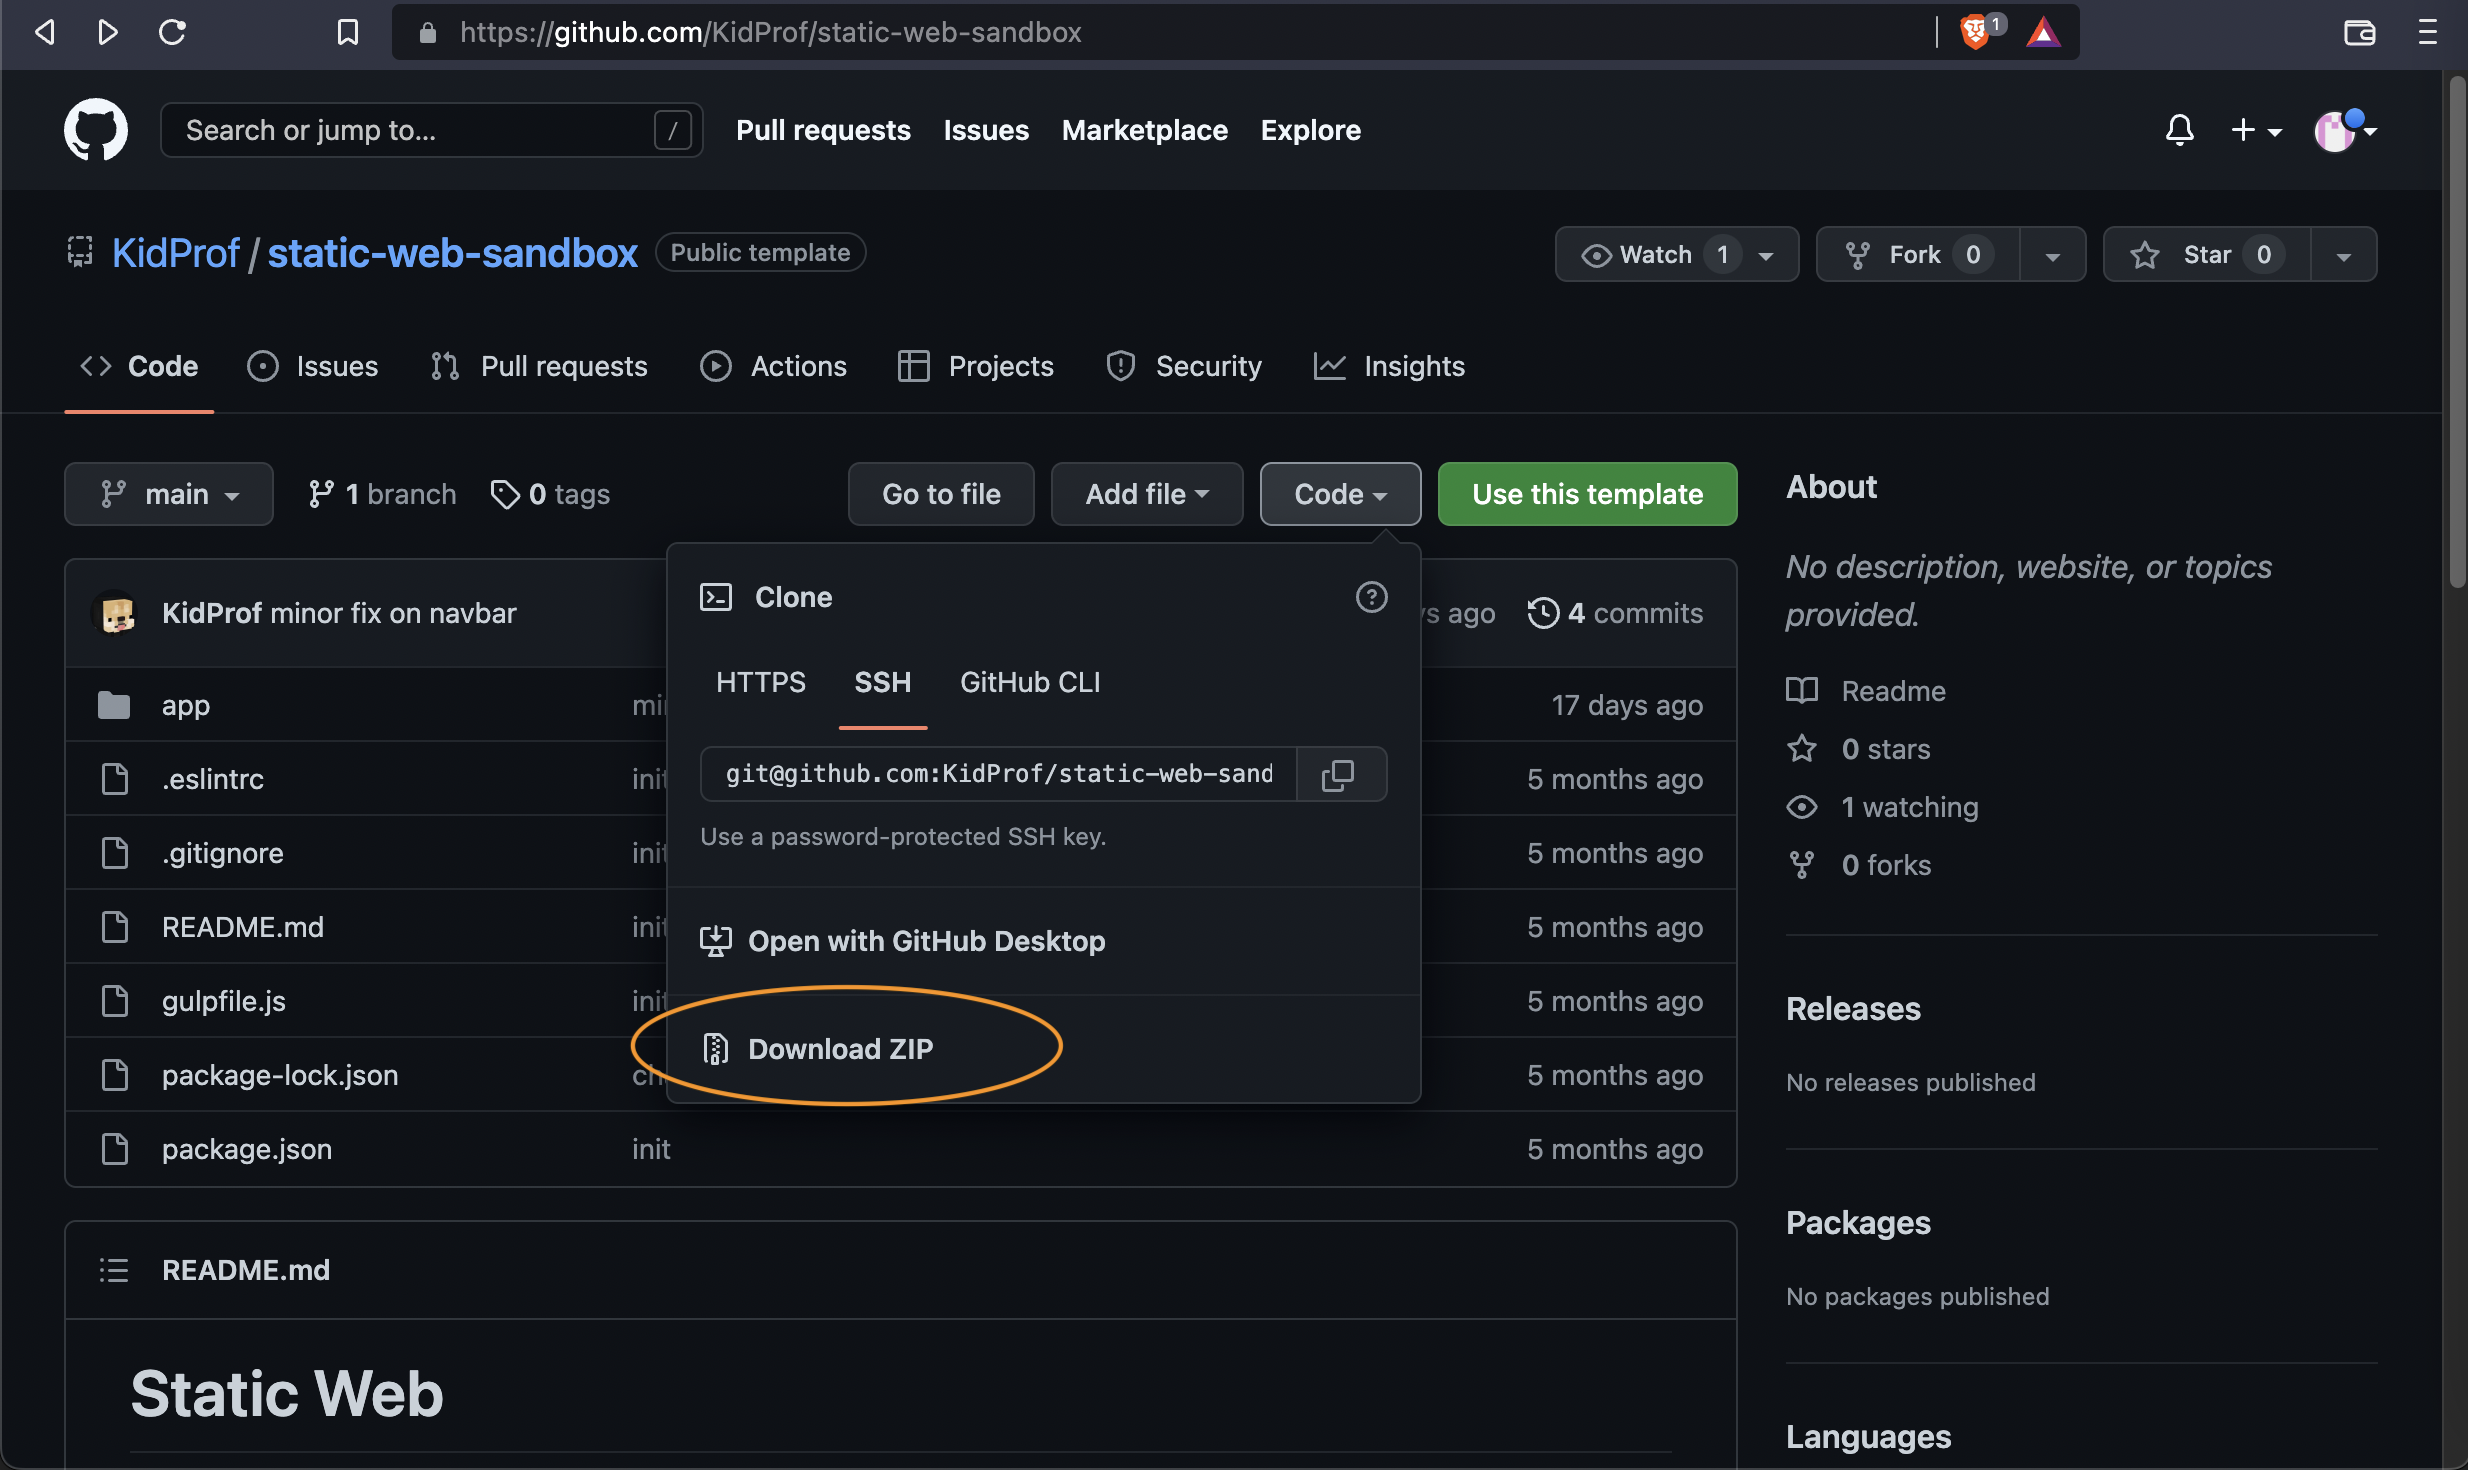
\includegraphics[width=15cm]{images/ch1-download-as-zip.png}
\caption{Screenshot from GitHub showing how to download the code by zip}
\end{figure}

\section{Git Bash (for Windows only)}
\label{sec:install1}

\textit{If you are using MacOS or Linux, skip to step 2: Creating a GitHub account}
\vspace{6mm}

Download Git Bash by following \href{https://git-scm.com/download/win}{this link}.\footnote{Link: \url{https://git-scm.com/download/win}} It should be straightforward.

\section{Creating a GitHub account}

Create your own GitHub account \href{https://github.com/}{here}.\footnote{Link: \url{https://github.com/}} It should be straightforward. Remember the email you used for registration.

\section{Creating a new repository using the template}

Open my template by following \href{https://github.com/KidProf/static-web-sandbox}{this link}.\footnote{Link: \url{https://github.com/KidProf/static-web-sandbox}} Then click the big green button \textit{Use this template}. You will be prompted to create a new repository. \textbf{Repository} is a fancier word for project, sometimes abbreviated to \textbf{repo}. Provide a repository name (a.k.a. project name) of your choice, preferably something meaningful; and you can set it either to public or private based on your own preference. You can change these two settings in the future. Do not change up any other settings in this page. \textit{(see figure)}

\begin{figure}[h]
\centering
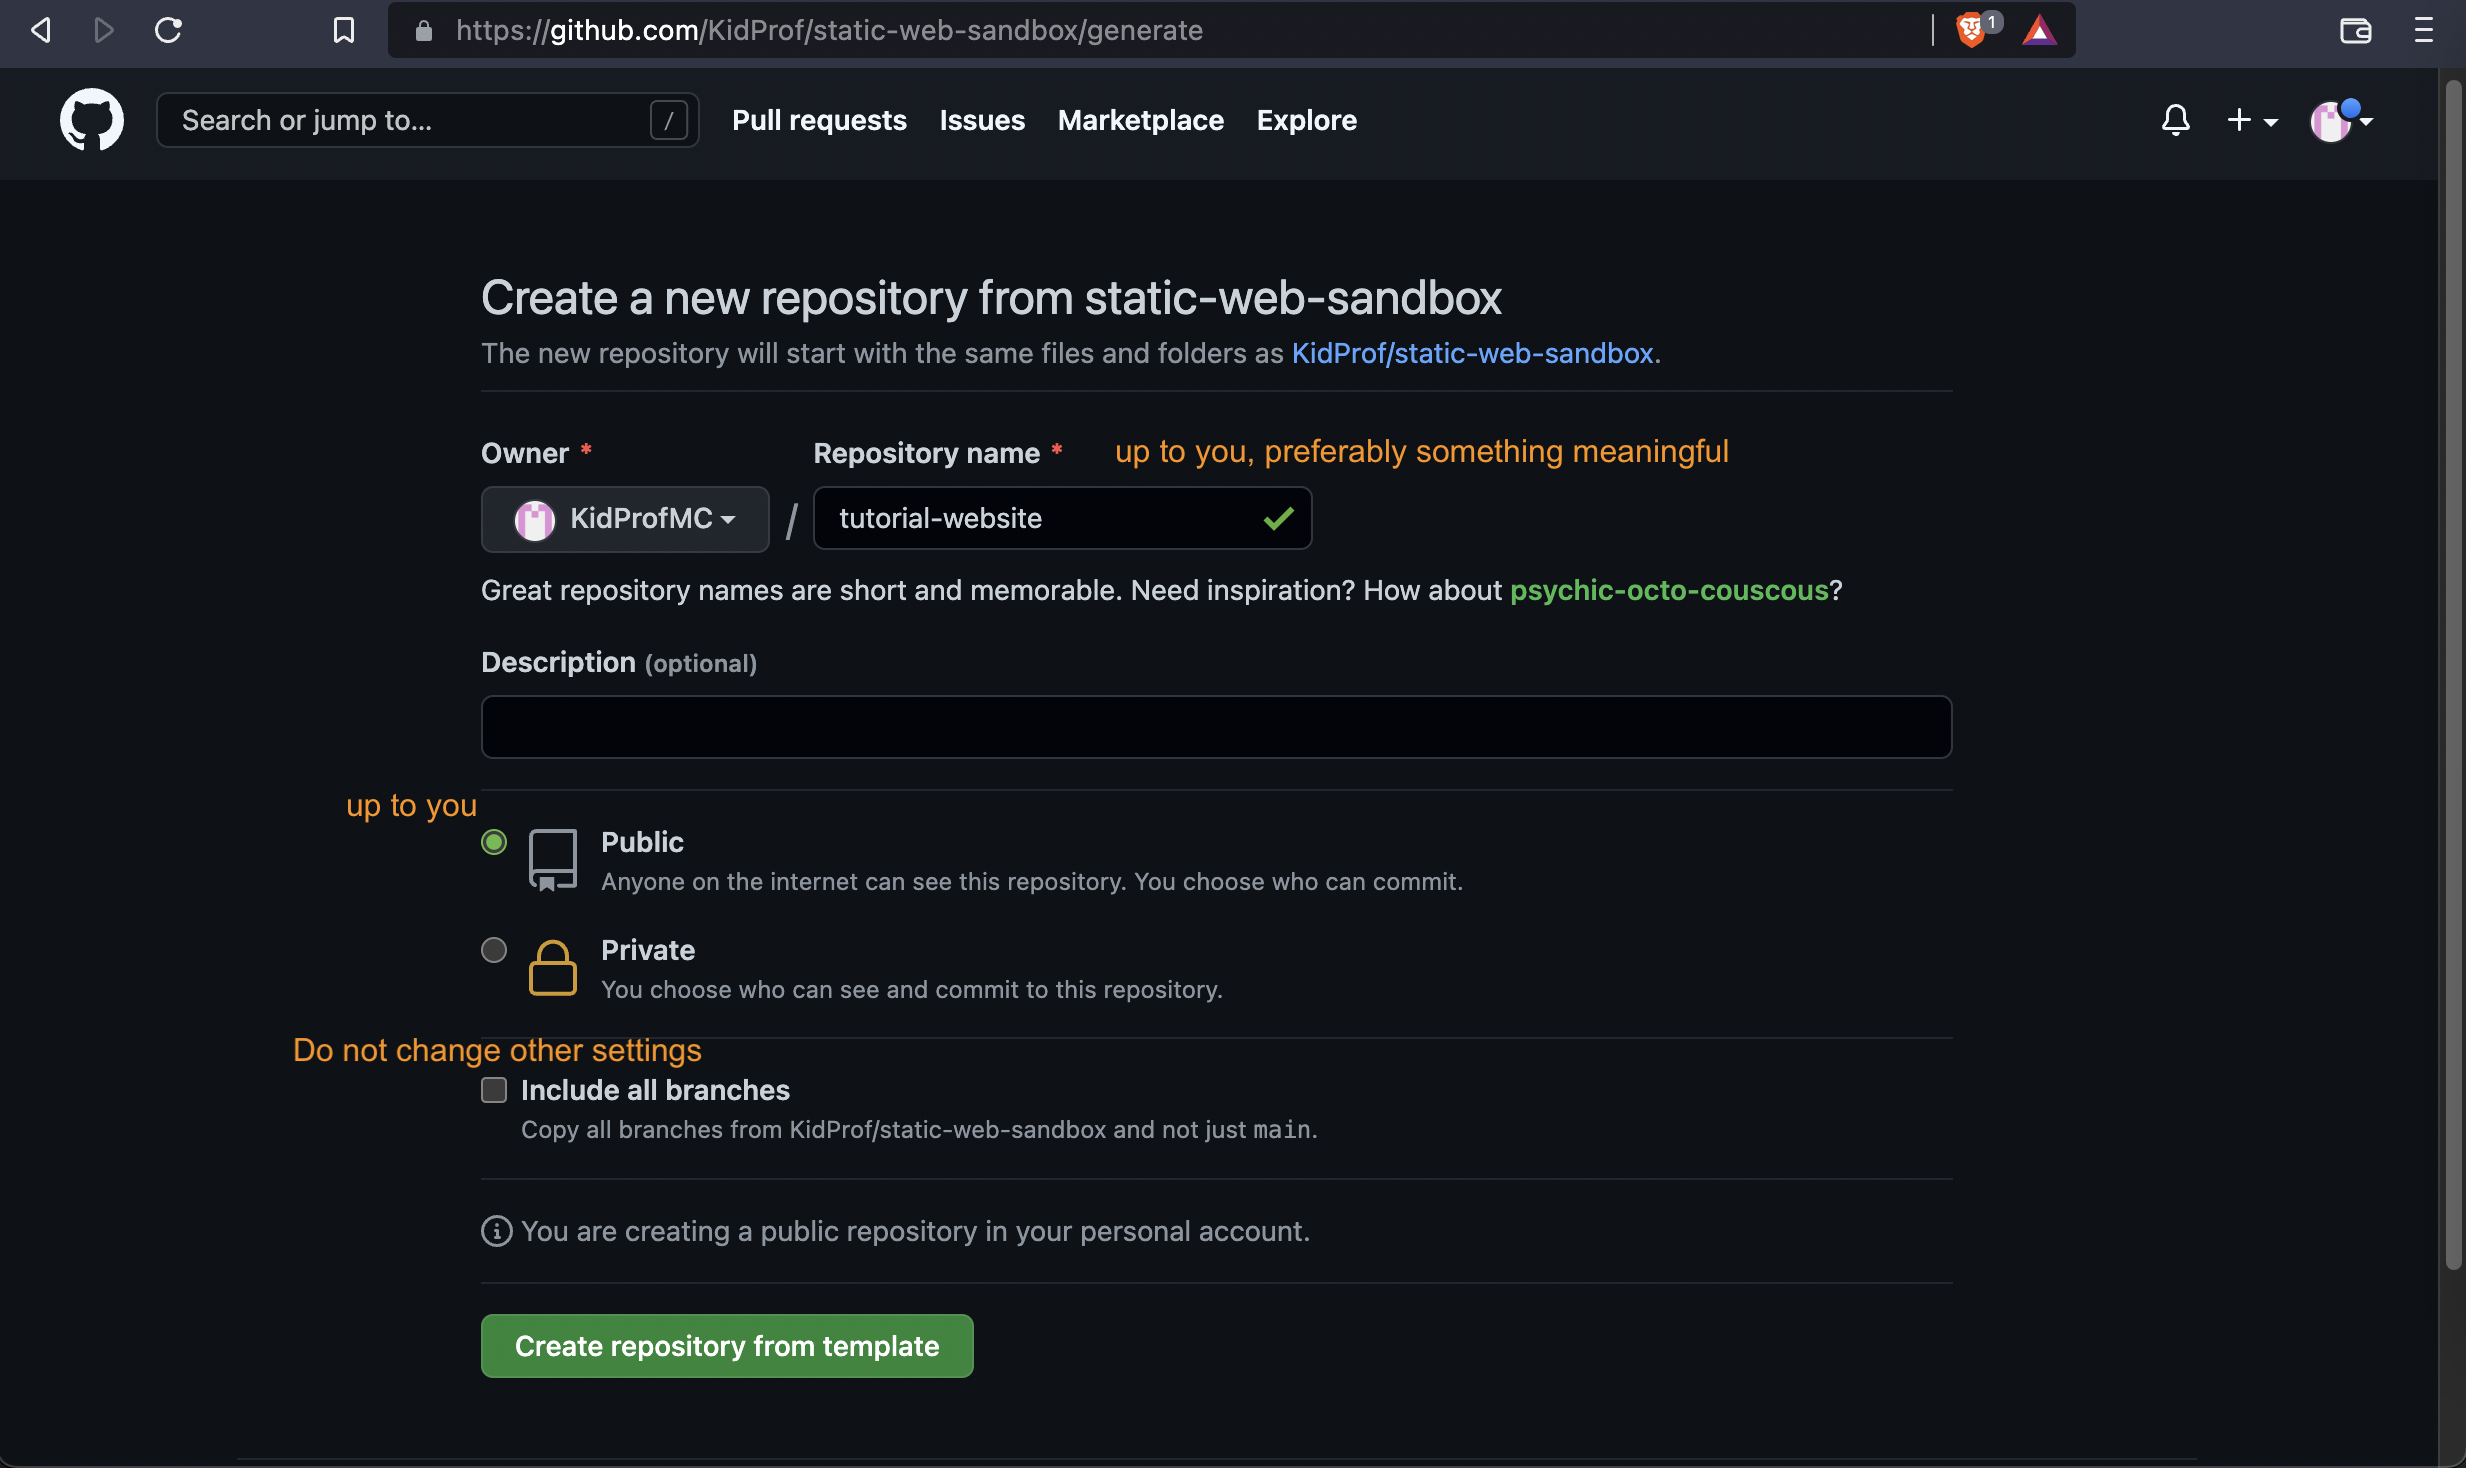
\includegraphics[width=15cm]{images/ch1-create-new-repo.png}
\caption{Creating a new repository}
\end{figure}

\section{Creating an SSH key}

An SSH key is to verify your identity on your local machine, so that you can access and manage your repositories on GitHub from your local machine.

Follow \href{https://docs.github.com/en/authentication/connecting-to-github-with-ssh/generating-a-new-ssh-key-and-adding-it-to-the-ssh-agent}{this tutorial}\footnote{Link: \url{https://docs.github.com/en/authentication/connecting-to-github-with-ssh/generating-a-new-ssh-key-and-adding-it-to-the-ssh-agent}}, then \href{https://docs.github.com/en/authentication/connecting-to-github-with-ssh/adding-a-new-ssh-key-to-your-github-account}{this tutorial}\footnote{Link: \url{https://docs.github.com/en/authentication/connecting-to-github-with-ssh/adding-a-new-ssh-key-to-your-github-account}}, and you are good to go. 
\vspace{6mm}

Use Git Bash if you are on a Windows machine, use the Terminal if you are on a MacOS or Linux machine. There is no need to understand and remember the commands, copying and pasting is one of the skills needed to be a good programmer. \textbf{The \$ symbol indicates the start of a command, so you do not need to copy the \$ symbol.}
\vspace{6mm}

For example, if I am using a Windows machine, I would run the following set of commands in my Git Bash line by line. Remember replace the email with your own email used to register for the GitHub account!

\begin{lstlisting}[language=bash]
$ ssh-keygen -t ed25519 -C "your_email@example.com"
$ eval "$(ssh-agent -s)"
$ ssh-add ~/.ssh/id_ed25519
$ clip < ~/.ssh/id_ed25519.pub
\end{lstlisting}

Then paste the SSH public key to the appropriate spot on the GitHub website according to the tutorials.

\section{Creating a folder using command line}
\label{sec:install5}

From now on, I would use the term \textbf{command line} to refer to Git Bash if you are on a Windows machine, and the Terminal if you are on a MacOS or Linux machine. 

So now open the command line, use \texttt{mkdir} followed by a folder name to create a new folder to store your code. Then, use \texttt{cd} followed by the folder name to enter to that folder.

\begin{lstlisting}[language=bash]
# KidProf in ~
$ mkdir code

# KidProf in ~
$ cd code

# KidProf in ~/code
$ 
\end{lstlisting}

\section{Downloading the code using SSH key}

Go back to your project on GitHub, click the big green button \textit{Code}, then remember to select \texttt{SSH}, then copy the URL given.

\begin{figure}[h]
\centering
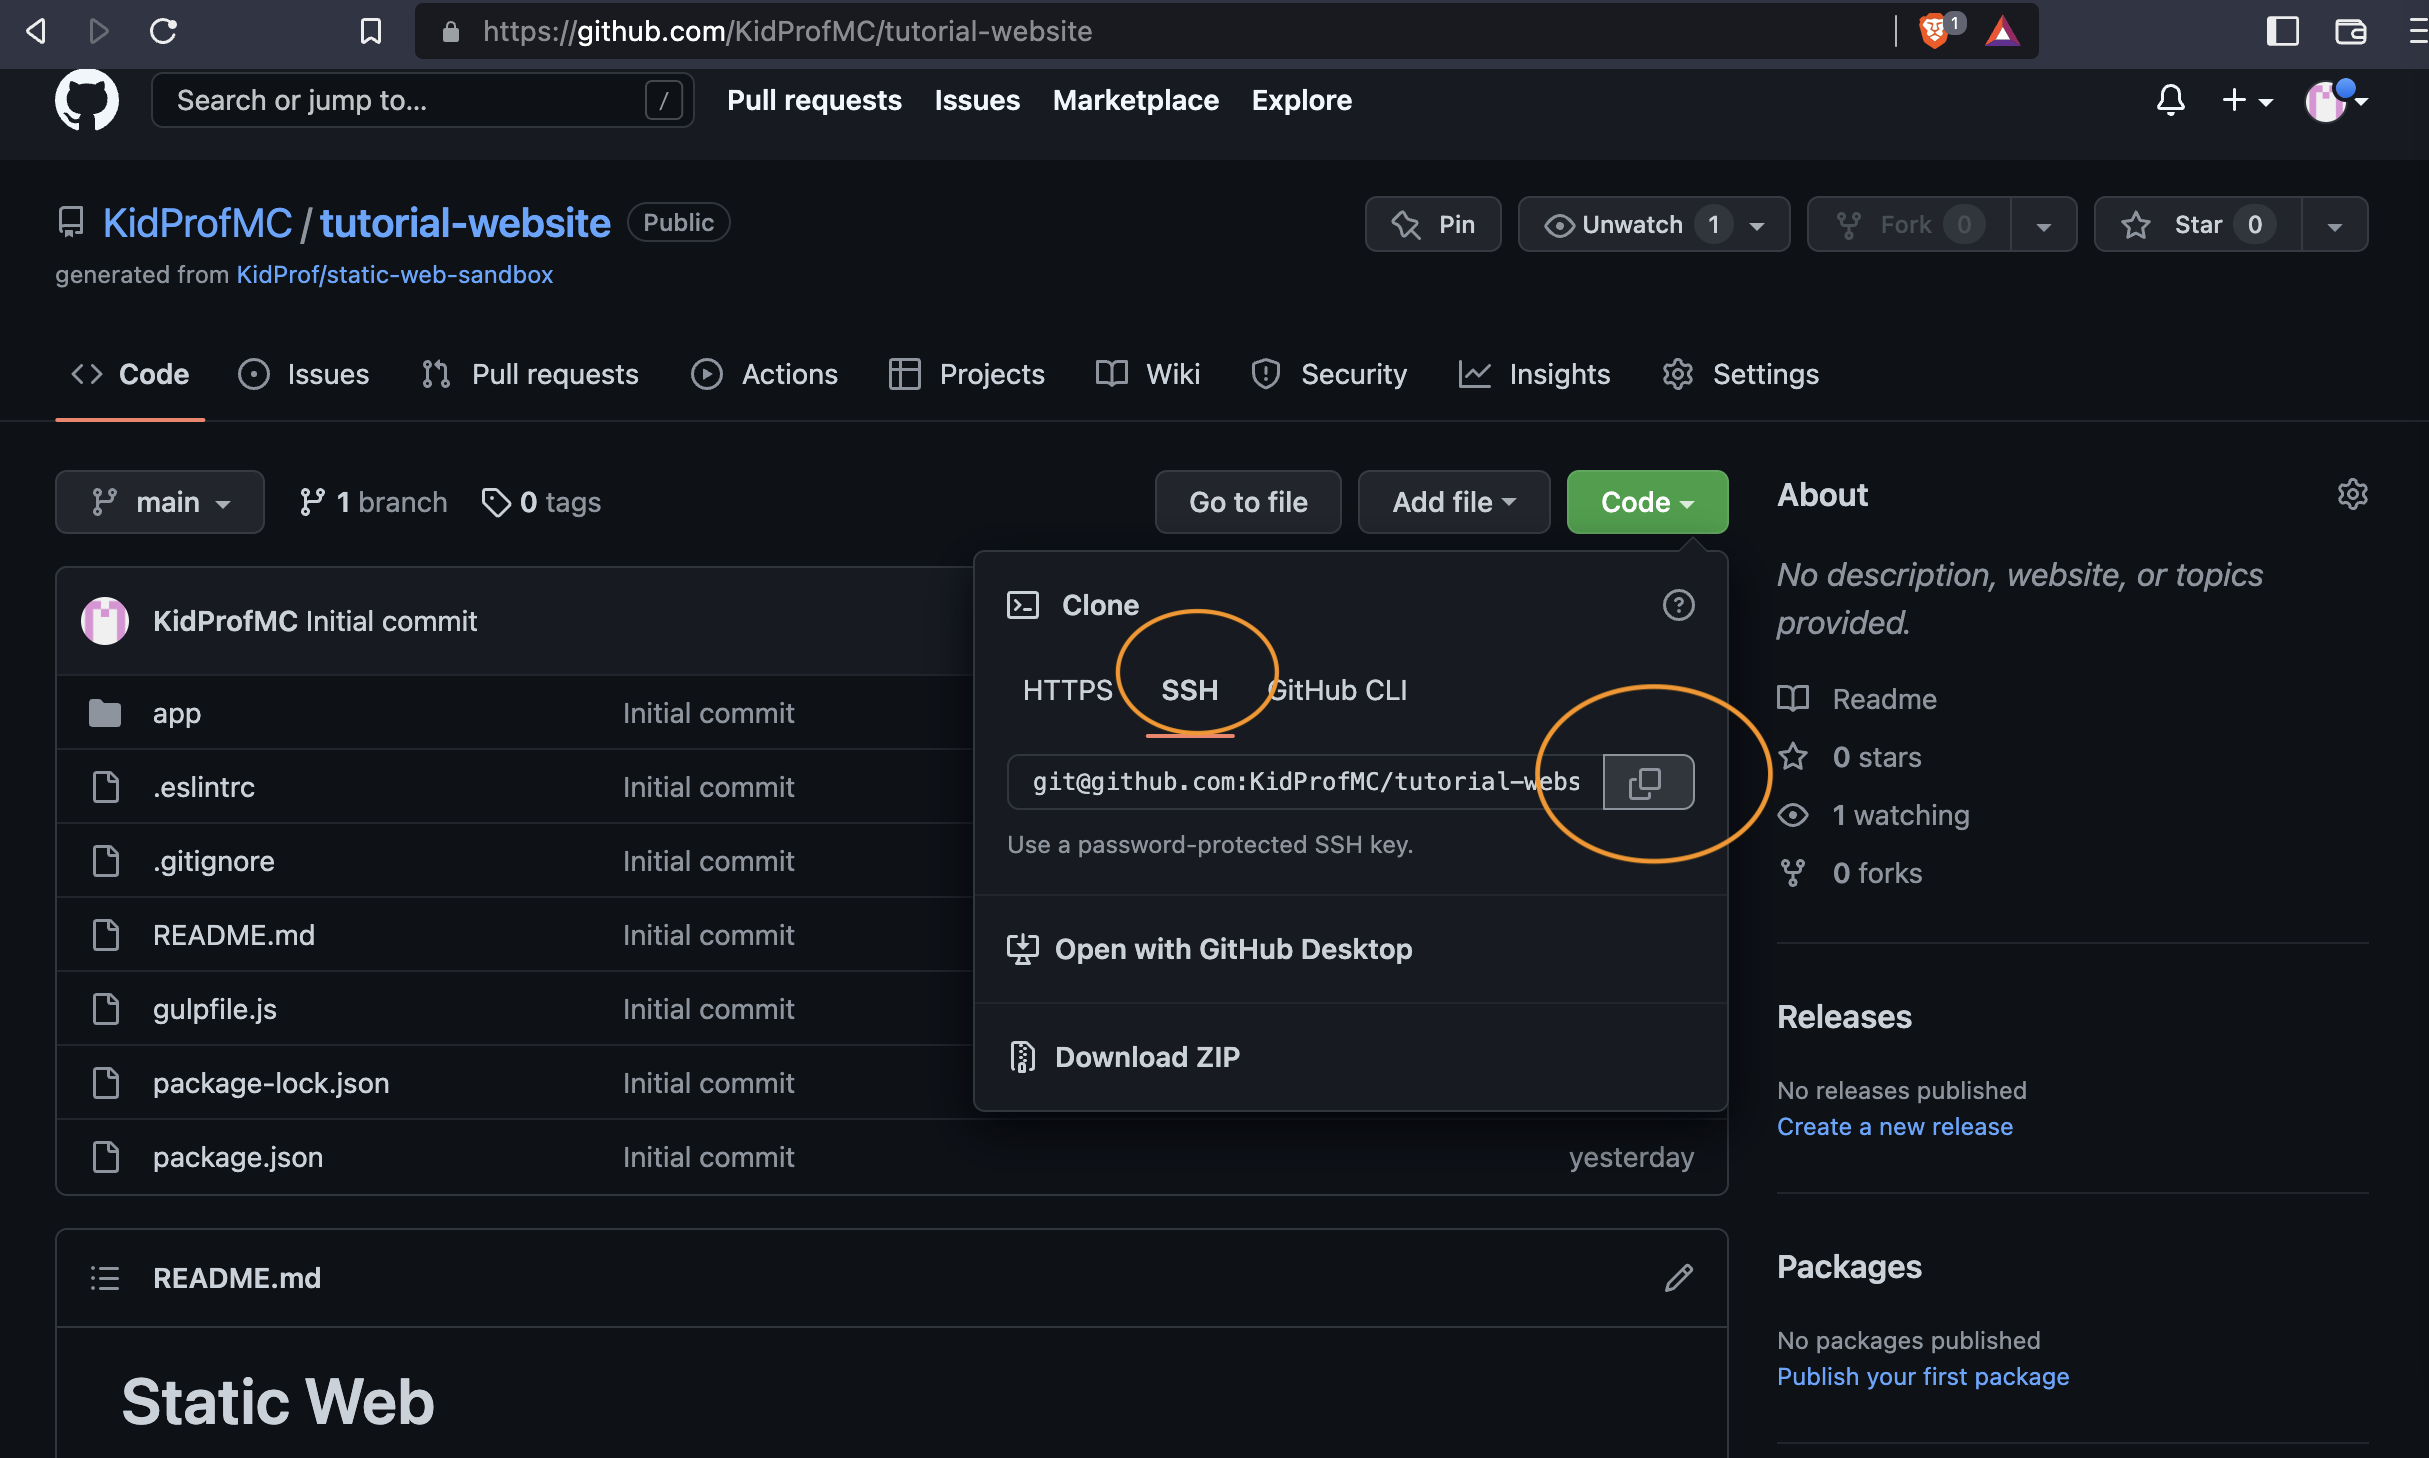
\includegraphics[width=15cm]{images/ch1-git-clone.png}
\caption{Getting the URL to download your project}
\end{figure}

Use \texttt{git clone}, followed by pasting the URL obtained from GitHub. You should use your mouse to paste the URL in the classic way, as \texttt{ctrl+V} would not work.

\section{Installing node.js}
\label{sec:install7}

Download node.js by following \href{https://nodejs.org/en/}{this link}.\footnote{Link: \url{https://nodejs.org/en/}} It should be straightforward. You should download the LTS\footnote{stands for long term support} version.

After installing, you can try running \texttt{node --version} in the command line.

\begin{lstlisting}[language=bash]
# If node is installed, it will show you the version number.
$ node --version
v16.14.0

# If node is not installed, it will show you an error message
$ node --version
zsh: command not found: node
\end{lstlisting}

\section{Installing dependencies for the project}

Open your command line, \texttt{cd} into the folder with the code in, run \texttt{npm install}. A new folder called \texttt{node\textunderscore modules} will be automatically created, with everything you need to use this project installed within that folder.

\begin{lstlisting}[language=bash]
# KidProf in ~
$ cd code

# KidProf in ~/code
$ cd tutorial-website

# KidProf in ~/code/tutorial-website
$ npm install
\end{lstlisting}

\section{Opening the web page}

Run \texttt{npm run build} to build the web page, more on this would be explained in \cref{sec:projstructure}.

Then, open the folder containing the project in file explorer/ finder. Go to the \texttt{docs} folder, open \texttt{index.html} using a web browser of your choice.

If you are unsure where your code is located, try running \texttt{pwd} in your command line, that should show you the full path that your code should be in.

\begin{lstlisting}[language=bash]
# KidProf in ~/code/tutorial-website on git:main 
$ npm run build

> static-web-sandbox@2.0.0 build
> gulp build

[09:56:22] Using gulpfile ~/code/tutorial-website/gulpfile.js
[09:56:22] Starting 'build'...
[09:56:22] Starting 'js'...
[09:56:22] Finished 'js' after 38 ms
[09:56:22] Starting 'pug'...
[09:56:22] Finished 'pug' after 83 ms
[09:56:22] Starting 'styling'...
[09:56:22] Finished 'styling' after 37 ms
[09:56:22] Starting 'imagecopy'...
[09:56:22] Finished 'imagecopy' after 2.67 ms
[09:56:22] Starting 'fontcopy'...
[09:56:22] Finished 'fontcopy' after 1.42 ms
[09:56:22] Finished 'build' after 164 ms

# KidProf in ~/code/tutorial-website on git:main 
$ pwd
/Users/KidProf/code/tutorial-website
\end{lstlisting}

\begin{figure}[h]
\centering
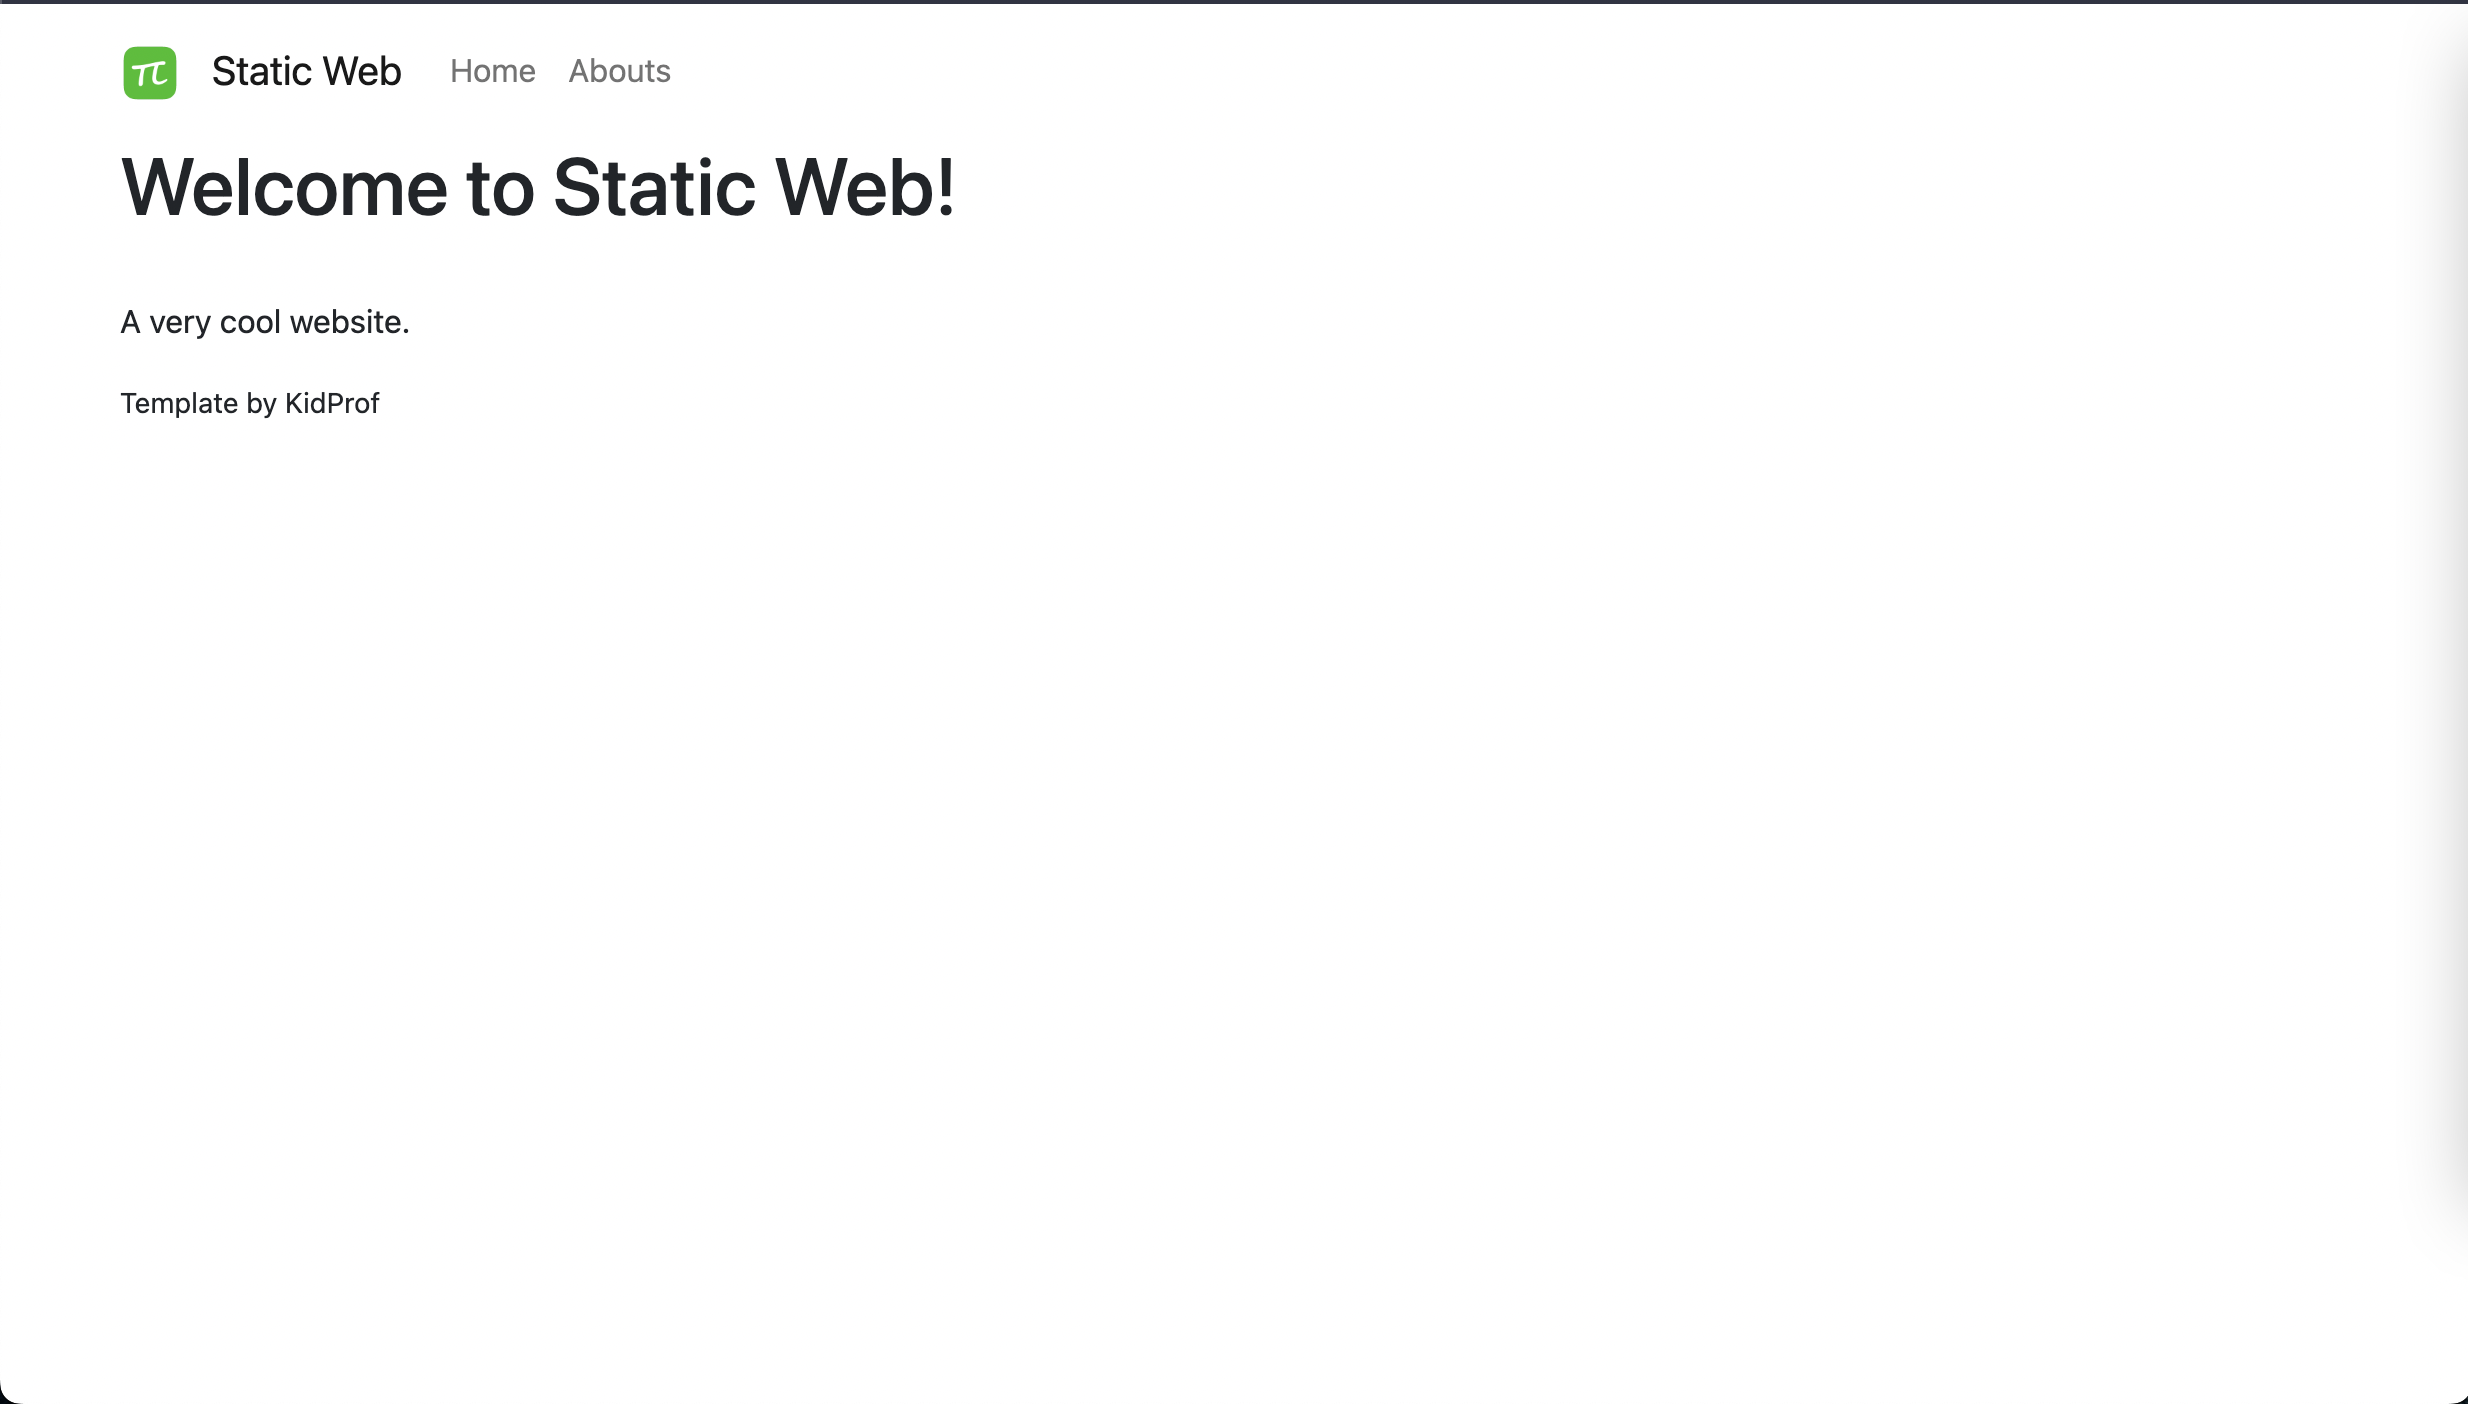
\includegraphics[width=15cm]{images/ch1-indexhtml.png}
\caption{What index.html should look like}
\end{figure}


\section{Installing VS Code}

Visual Studio Code (VS Code) is a text editor, with highlighted syntax and many more user-friendly features for you to code efficiently.

Download VS Code by following \href{https://code.visualstudio.com/}{this link}.\footnote{Link: \url{https://code.visualstudio.com/}} It should be straightforward.

\label{sec:pwdch1}
Then, open VS Code and open the folder containing the code. If you are unsure where your code is located, try running \texttt{pwd} in your command line, that should show you the full path that your code should be in.

There are a number of extensions available in VS Code, but I think they are not necessary for beginners.
\vspace{6mm}

This marks the end of the installation marathon. I hope you have learned some basic command line commands along the way, we will formally introduce them in \hyperref[sec:cmd]{the next chapter.}

\chapter{Command Line}

\section{Basic commands}

\textit{Covered in \href{https://www.youtube.com/watch?v=oIsH0V3fRt8&list=PLjGmdnqrOKuYXiu7lgG5HW71jPEUd1XCm&index=2}{video 1 of the series}}

\subsection{\texttt{ls}}

\texttt{ls} stands for list. Lists out the files and folders you have in your current directory. \textbf{Directory is another word for folder.}

\begin{lstlisting}[language=bash]
$ ls
README.md   docs  node_modules  package.json    
app     gulpfile.js     package-lock.json
\end{lstlisting}

You could run \texttt{ls -a} to show hidden files and folders as well, which are the ones with their names start with a \texttt{.}

\begin{lstlisting}[language=bash]
$ ls -a
.   .git    docs    package.json
..  .gitignore  gulpfile.js
.DS_Store   README.md   node_modules
.eslintrc   app package-lock.json
\end{lstlisting}

As you can see a hidden folder \texttt{.git} and a hidden file \texttt{.gitignore} are displayed.

\subsection{\texttt{cd}}

\texttt{cd} stands for change directory, self explanatory ;). Use \texttt{cd ..} to go back to the previous directory (to go out one folder). 

\begin{lstlisting}[language=bash]
# KidProf in ~
$ cd code

# KidProf in ~/code
$ cd ..

# KidProf in ~
\end{lstlisting}

\subsection{\texttt{pwd}}

\texttt{pwd} shows the current directory you are in in full. As shown in chapter1 it makes it easier for you to locate our work folder in Finder/ File Explorer.

\begin{lstlisting}[language=bash]
# KidProf in ~
$ pwd
/Users/KidProf
\end{lstlisting}

\subsection{\texttt{touch}}

Creates a new file. For example, \texttt{touch test.txt}

\subsection{\texttt{mkdir}}

Creates a new folder. For example, \texttt{mkdir code}

\subsection{\texttt{--version}}

To check the version of a certain software. It is commonly used to verify that you have installed the software correctly. 

\begin{lstlisting}[language=bash]
(node is installed)
$ node --version
v16.14.0

(node is not installed)
$ node --version
bash: command not found: node
\end{lstlisting}

\section{A word on directories}

\texttt{.} refers to the current directory.

\texttt{..} refers to the previous directory.

\texttt{$\sim$} refers to the home directory, it is the initial directory when you open the command line. In the \texttt{pwd} example, you can see the home directory of my Mac is \texttt{/Users/KidProf}. You should do most of your work inside this home directory. To go back to the home directory, do \texttt{cd $\sim$} This is useful when you get stuck in some other directories.

When the path is not prepended with a \texttt{/}, it is a relative path. Meaning that it is relative to the current directory.

When the path is prepended with a \texttt{/}, it is an absolute path. 

\begin{lstlisting}[language=bash]
(cd to an relative path)
# KidProf in ~
$ cd code

# KidProf in ~/code

(cd to an absolute path)
# KidProf in ~
$ cd /Users/KidProf/code

# KidProf in ~/code
\end{lstlisting}

\section{General Tips}

\textit{Covered in \href{https://www.youtube.com/watch?v=oIsH0V3fRt8&list=PLjGmdnqrOKuYXiu7lgG5HW71jPEUd1XCm&index=2}{video 1 of the series}}
\vspace{6mm}

Use up and down arrow to navigate your command history. Very useful when you are calling the same command repeatedly or when you made some typos.

Press \texttt{ctrl+C} to .... % TODO

\section{More commands}

\textit{Advanced, }
\textit{covered in \href{https://www.youtube.com/watch?v=ZIBEVGrtiVA&list=PLjGmdnqrOKuYXiu7lgG5HW71jPEUd1XCm&index=7}{video 6a of the series}}
\vspace{6mm}

\subsection{\texttt{cp}}

\subsection{\texttt{rm}}

\subsection{\texttt{mv}}

\section{Vim - command line text editor}

\textit{Advanced}
\vspace{6mm}

The default text editor is called Vim. It may appear when you run some commands that require messages to be inputted, for example, \texttt{git commit} \textit{(More in Chapter 3)}.

Unfortunately, it is quite difficult to use and needs some time to get used to. So I tried my best to provide alternative commands that prevent this text editor from popping up, for example, using \texttt{git commit -m "message"}

However, here are the basics of using Vim, so that you will not get too lost when you encounter it. You can practice by entering \texttt{vim} in the command line.

You start in a mode called "normal mode". You can’t immediately type anything.

In order to get typing press \texttt{i} (stands for insert). This will bring you to "insert mode", so named because in this mode you can actually type.

When you are done typing press \texttt{esc}. This will bring you back to "normal mode".

In order to save your work you want to type :w and press return. And in order to exit vim you want to type \texttt{:q} and press return. Because saving and quitting is a very common action, there is actually a shortcut \texttt{:x}, which stands for \texttt{:wq} (which just combines \texttt{:w} and \texttt{:q}).\footnote{Reference: \url{https://web.mit.edu/6.005/www/fa14/tutorial/git/config.html}}


If you do not wish to save the file, you can use \texttt{:q!}



\chapter{Git}
\label{sec:ch3}
Git is important because it allows you to work and communicate with people using just a few simple commands. By following its rules and conventions, you can work with others efficiently, without having to send zip files back and forth through emails. It also allows version control, for you to keep track of changes you have made to your code, and revert to a previous version or take reference from your previous changes when necessary.
\vspace{6mm}

We will focus on getting Git set up and basic commands in this chapter. After reading this chapter, you will be able to use Git alone for version control, as if it is a save button of your work. A few more commands will be introduced in \cref{sec:git2} to allow you to work with others.

\begin{center}

\includegraphics[width=10cm]{images/ch0-version-control.jpeg}
\end{center}

\section{Git VS GitHub}

Before we start, it is a good idea to distinguish between Git and GitHub. Git runs on your local machine, keeping track of the changes you have made locally. While GitHub is a cloud service provider\footnote{There are also other similar cloud service provider but GitHub is the most popular one}, keeping track of changes made to different people. That version of the project on GitHub should be the one that all local machines follow.

\begin{center}
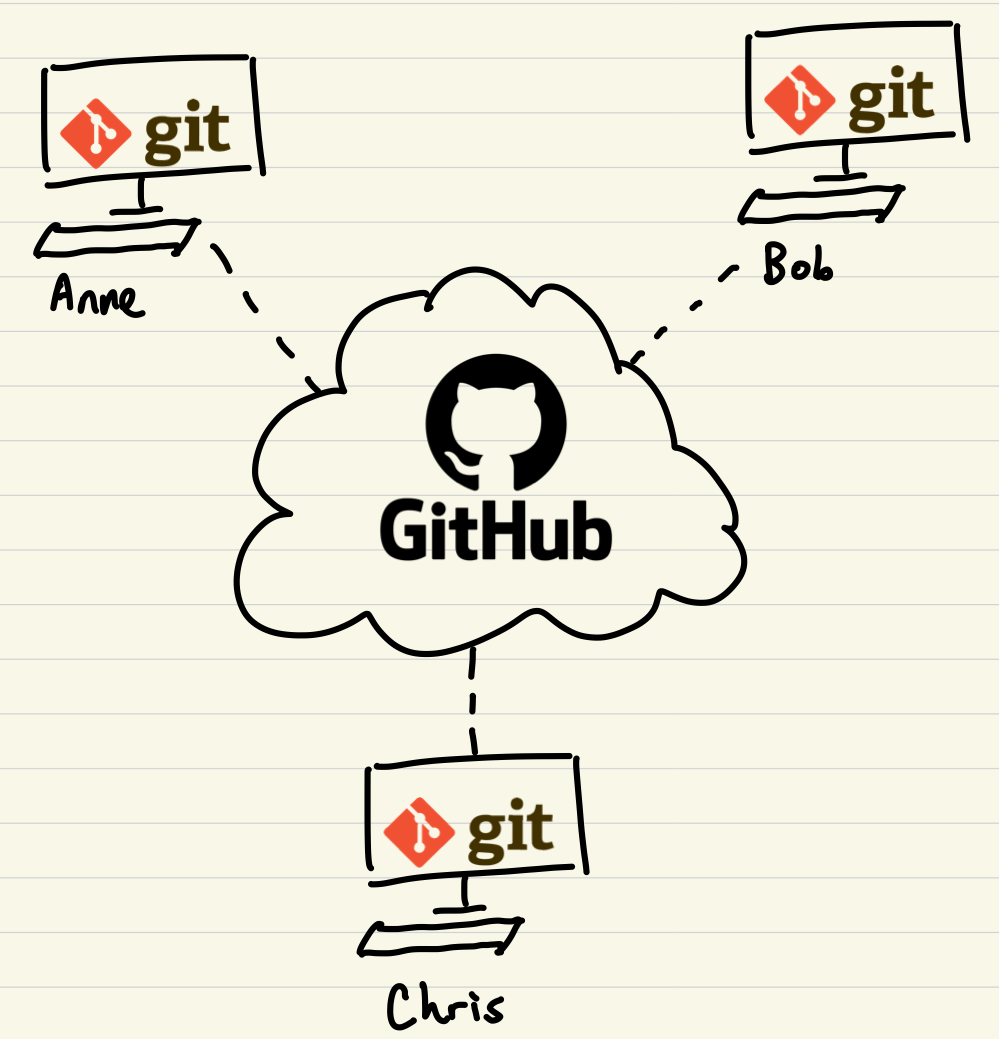
\includegraphics[width=10cm]{images/ch3-gitgithub.png}
\end{center}

\section{First time using Git}
\label{sec:gitfirst}

\textit{Covered in \href{https://www.youtube.com/watch?v=wQmFz-Ggxuo&list=PLjGmdnqrOKuYXiu7lgG5HW71jPEUd1XCm&index=4}{video 3 of the series}}
\vspace{6mm}

Let's just change out \texttt{app/templates/views/index.pug} slightly so that we can make our first push to GitHub. Or if you are working on other projects, you can pick a random file and made some edits.

\begin{lstlisting}[language=pug]
//- app/templates/views/index.pug
extends ../layouts/default

block content
	.container
		h1 Welcome to Static Web!
		br
		p A very cool website.
		p This web is made for tutorial purposes.
\end{lstlisting}

One very useful command - \texttt{git status} displays information about current situation, it might also contains some hints on which command(s) you need to run to proceed.

\begin{lstlisting}[language=bash]
$ git status
On branch main
Your branch is up to date with 'origin/main'.

Changes not staged for commit:
  (use "git add <file>..." to update what will be committed)
  (use "git restore <file>..." to discard changes in working directory)
	modified:   app/templates/views/index.pug

no changes added to commit (use "git add" and/or "git commit -a")
\end{lstlisting}

\subsection*{First add}
So you can see it is prompting you to run \texttt{git add <file>}. Instead, I would prefer \texttt{git add .} As discussed in \cref{sec:dir}, \texttt{.} refers to the current directory. That means, we are adding all the changes in the folder to be ready for a commit.

\begin{lstlisting}[language=bash]
$ git add .
\end{lstlisting}

Then, run \texttt{git status} again to asset the situation. The modified file should now be highlighted in green. (sadly you cannot see the green highlighting in LaTeX)

\begin{lstlisting}[language=bash]
$ git status
On branch main
Your branch is up to date with 'origin/main'.

Changes to be committed:
  (use "git restore --staged <file>..." to unstage)
	modified:   app/templates/views/index.pug
\end{lstlisting}

\subsection*{First commit (and set up your name and email)}

Next step, we are now ready to commit. \texttt{git commit} seals and confirms your changes into one chunk, and adds a commit message. The \textbf{commit message} should be meaningful, summarising what you have achieved with these code changes.

\begin{lstlisting}[language=]
$ git commit -m "experimenting with git"
[main e7bc529] experimenting with git
Committer: KidProf <kidprof@KidProfs-MacBook-Air.local>
Your name and email addresses were configured automatically
...
git config --global --edit
git config --amend --reset-author
1 file changed, 2 insertions(+), 1 deletion(-)
\end{lstlisting}

We got a problem here, our username and email do not match with the ones on GitHub. We need to \#1) change the default name and email on our device, and \#2) change the name and email for this particular commit.

Instead of the commands recommended automatically by Git, I recommend variants of those commands which are listed below, because these commands won't trigger the command line text editor to pop up. (see \cref{sec:vim})

Run the following two commands for \#1, replace with your own ones. Surround your name with double quotes if your name contains spaces.

\begin{lstlisting}[language=bash]
$ git config --global user.name KidProf
$ git config --global user.email kidprof@gmail.com
\end{lstlisting}

To verify, rerun those two commands but without the name and email, it should display your name and email as output.

\begin{lstlisting}[language=bash]
$ git config --global user.name
KidProf
$ git config --global user.email
kidprof@gmail.com
\end{lstlisting}

This command is for \#2.

\begin{lstlisting}[language=bash]
$ git config --amend --reset-author --no-edit
\end{lstlisting}

All set, now try running \texttt{git status} again.

\begin{lstlisting}[language=]
$ git status
On branch main
Your branch is ahead of 'origin/main' by 1 commit.
  (use "git push" to publish your local commits)

nothing to commit, working tree clean
\end{lstlisting}

\subsection*{First push}

Time to run \texttt{git push}, our last step. Except it might return an error.

\begin{lstlisting}[language=]
$ git push
fatal: The current branch main has no upstream branch.
To push the current branch and set the remote as upstream, use

    git push --set-upstream origin main
\end{lstlisting}

This one is quite an easy fix, just run the substitute command as instructed. You will need this whenever you are pushing a new branch to GitHub. \texttt{git push} should be sufficient for subsequent pushes.

\begin{lstlisting}[language=]
$ git push --set-upstream origin main
Enumerating objects: 11, done.
Counting objects: 100% (11/11), done.
Delta compression using up to 8 threads
Compressing objects: 100% (6/6), done.
Writing objects: 100% (6/6), 575 bytes | 575.00 KiB/s, done.
Total 6 (delta 3), reused 0 (delta 0), pack-reused 0
remote: Resolving deltas: 100% (3/3), completed with 3 local objects.
To github.com:KidProfMC/tutorial-website.git
\end{lstlisting}

\begin{center}
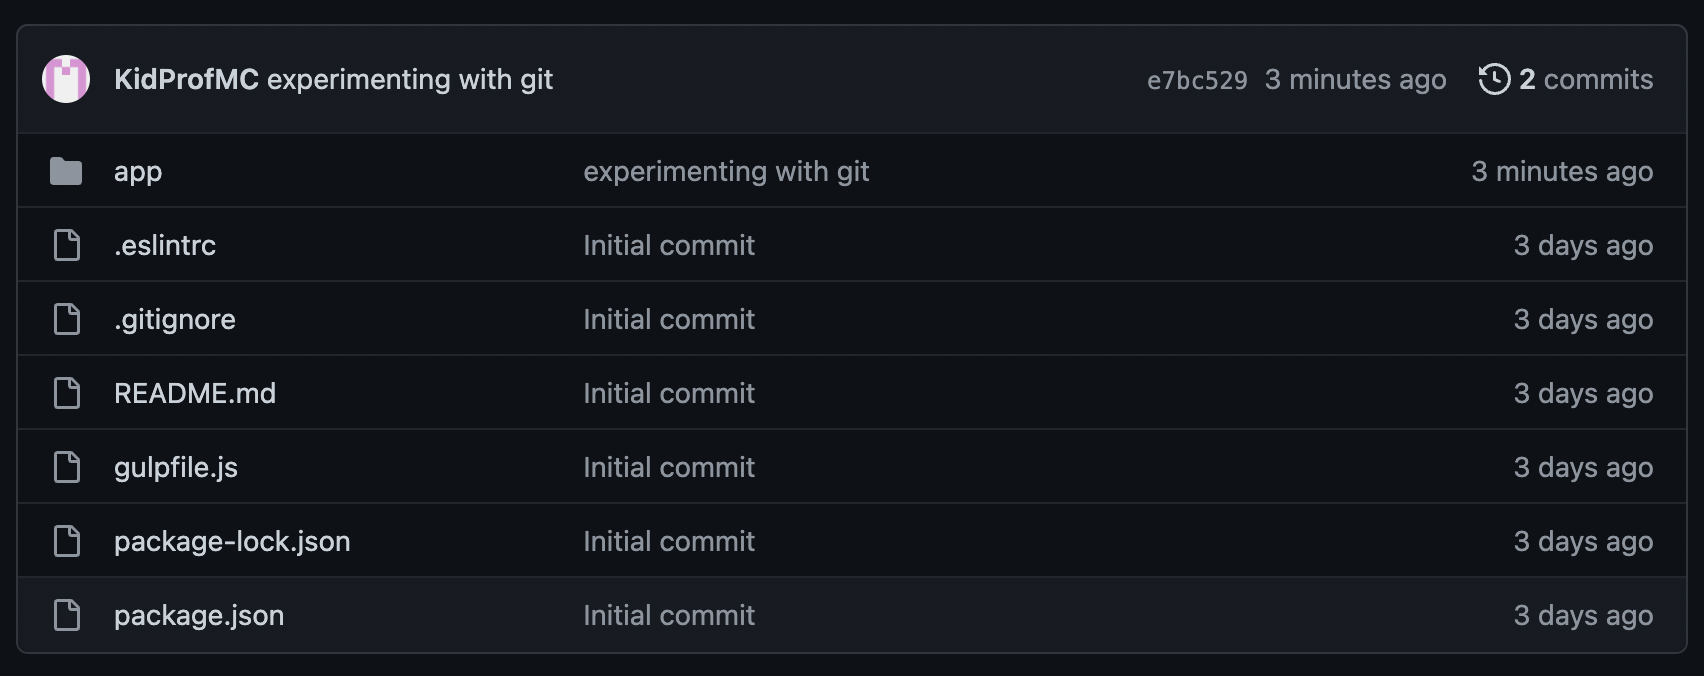
\includegraphics[width=12cm]{images/ch3-firstpushsuccess.png}
\end{center}

There you go, that is the first push. I will not list out the results of \texttt{git status} anymore in future sections, because they are taking too much space, but bear in mind running \texttt{git status} regularly is very useful.

\section{A typical day using Git}
\label{sec:gcmsg}

\textit{Covered in \href{https://www.youtube.com/watch?v=wQmFz-Ggxuo&list=PLjGmdnqrOKuYXiu7lgG5HW71jPEUd1XCm&index=4}{video 3 of the series}}
\vspace{6mm}

It is much more regular after the first push. You just need to remember three steps, add, commit and push.

\begin{lstlisting}[language=bash]
$ git add .
$ git commit -m "your message here"
$ git push
\end{lstlisting}

\texttt{git add} adds the changes you have made to be ready for the commit. 

\texttt{git commit} seals and confirms your changes into one chunk, and adds a commit message. The \textbf{commit message} should be meaningful, summarising what you have achieved with these code changes.

\texttt{git push} uploads the commit from your local machine to GitHub. \textbf{Push} is another fancier word for upload
\vspace{6mm}

You should perform these three steps whenever you have made some progress on your code, as if it is a save button. Practice makes perfect!

\subsection*{When do I have to set name and email like in the previous section?}

Every time you are using a new computer.

\subsection*{When do I have to add \texttt{--set-upstream} when pushing?}

Every time you are pushing a new branch to GitHub. You don't need to remember to do so because Git will reminds you anyways as shown in the previous section.

\section{Visualising}
\label{sec:sublime}
Git is a command line tool and is best used through the command line. Again, you will come across some situations where only command line is available (e.g. when accessing a remote server). 

However, it is acceptable if you just want to visualise the git commit history. Just don't run any commands using them. The following are two software recommended by me to do so. Sublime Merge looks nicer while Git Graph is visible inside VS Code. 

\subsection*{Sublime Merge}

Download Sublime Merge by following \href{https://www.sublimemerge.com/}{this link}.\footnote{Link: \url{https://www.sublimemerge.com/}} It should be straightforward. 

After installing, open the repository folder. The commit history is displayed.

\begin{center}
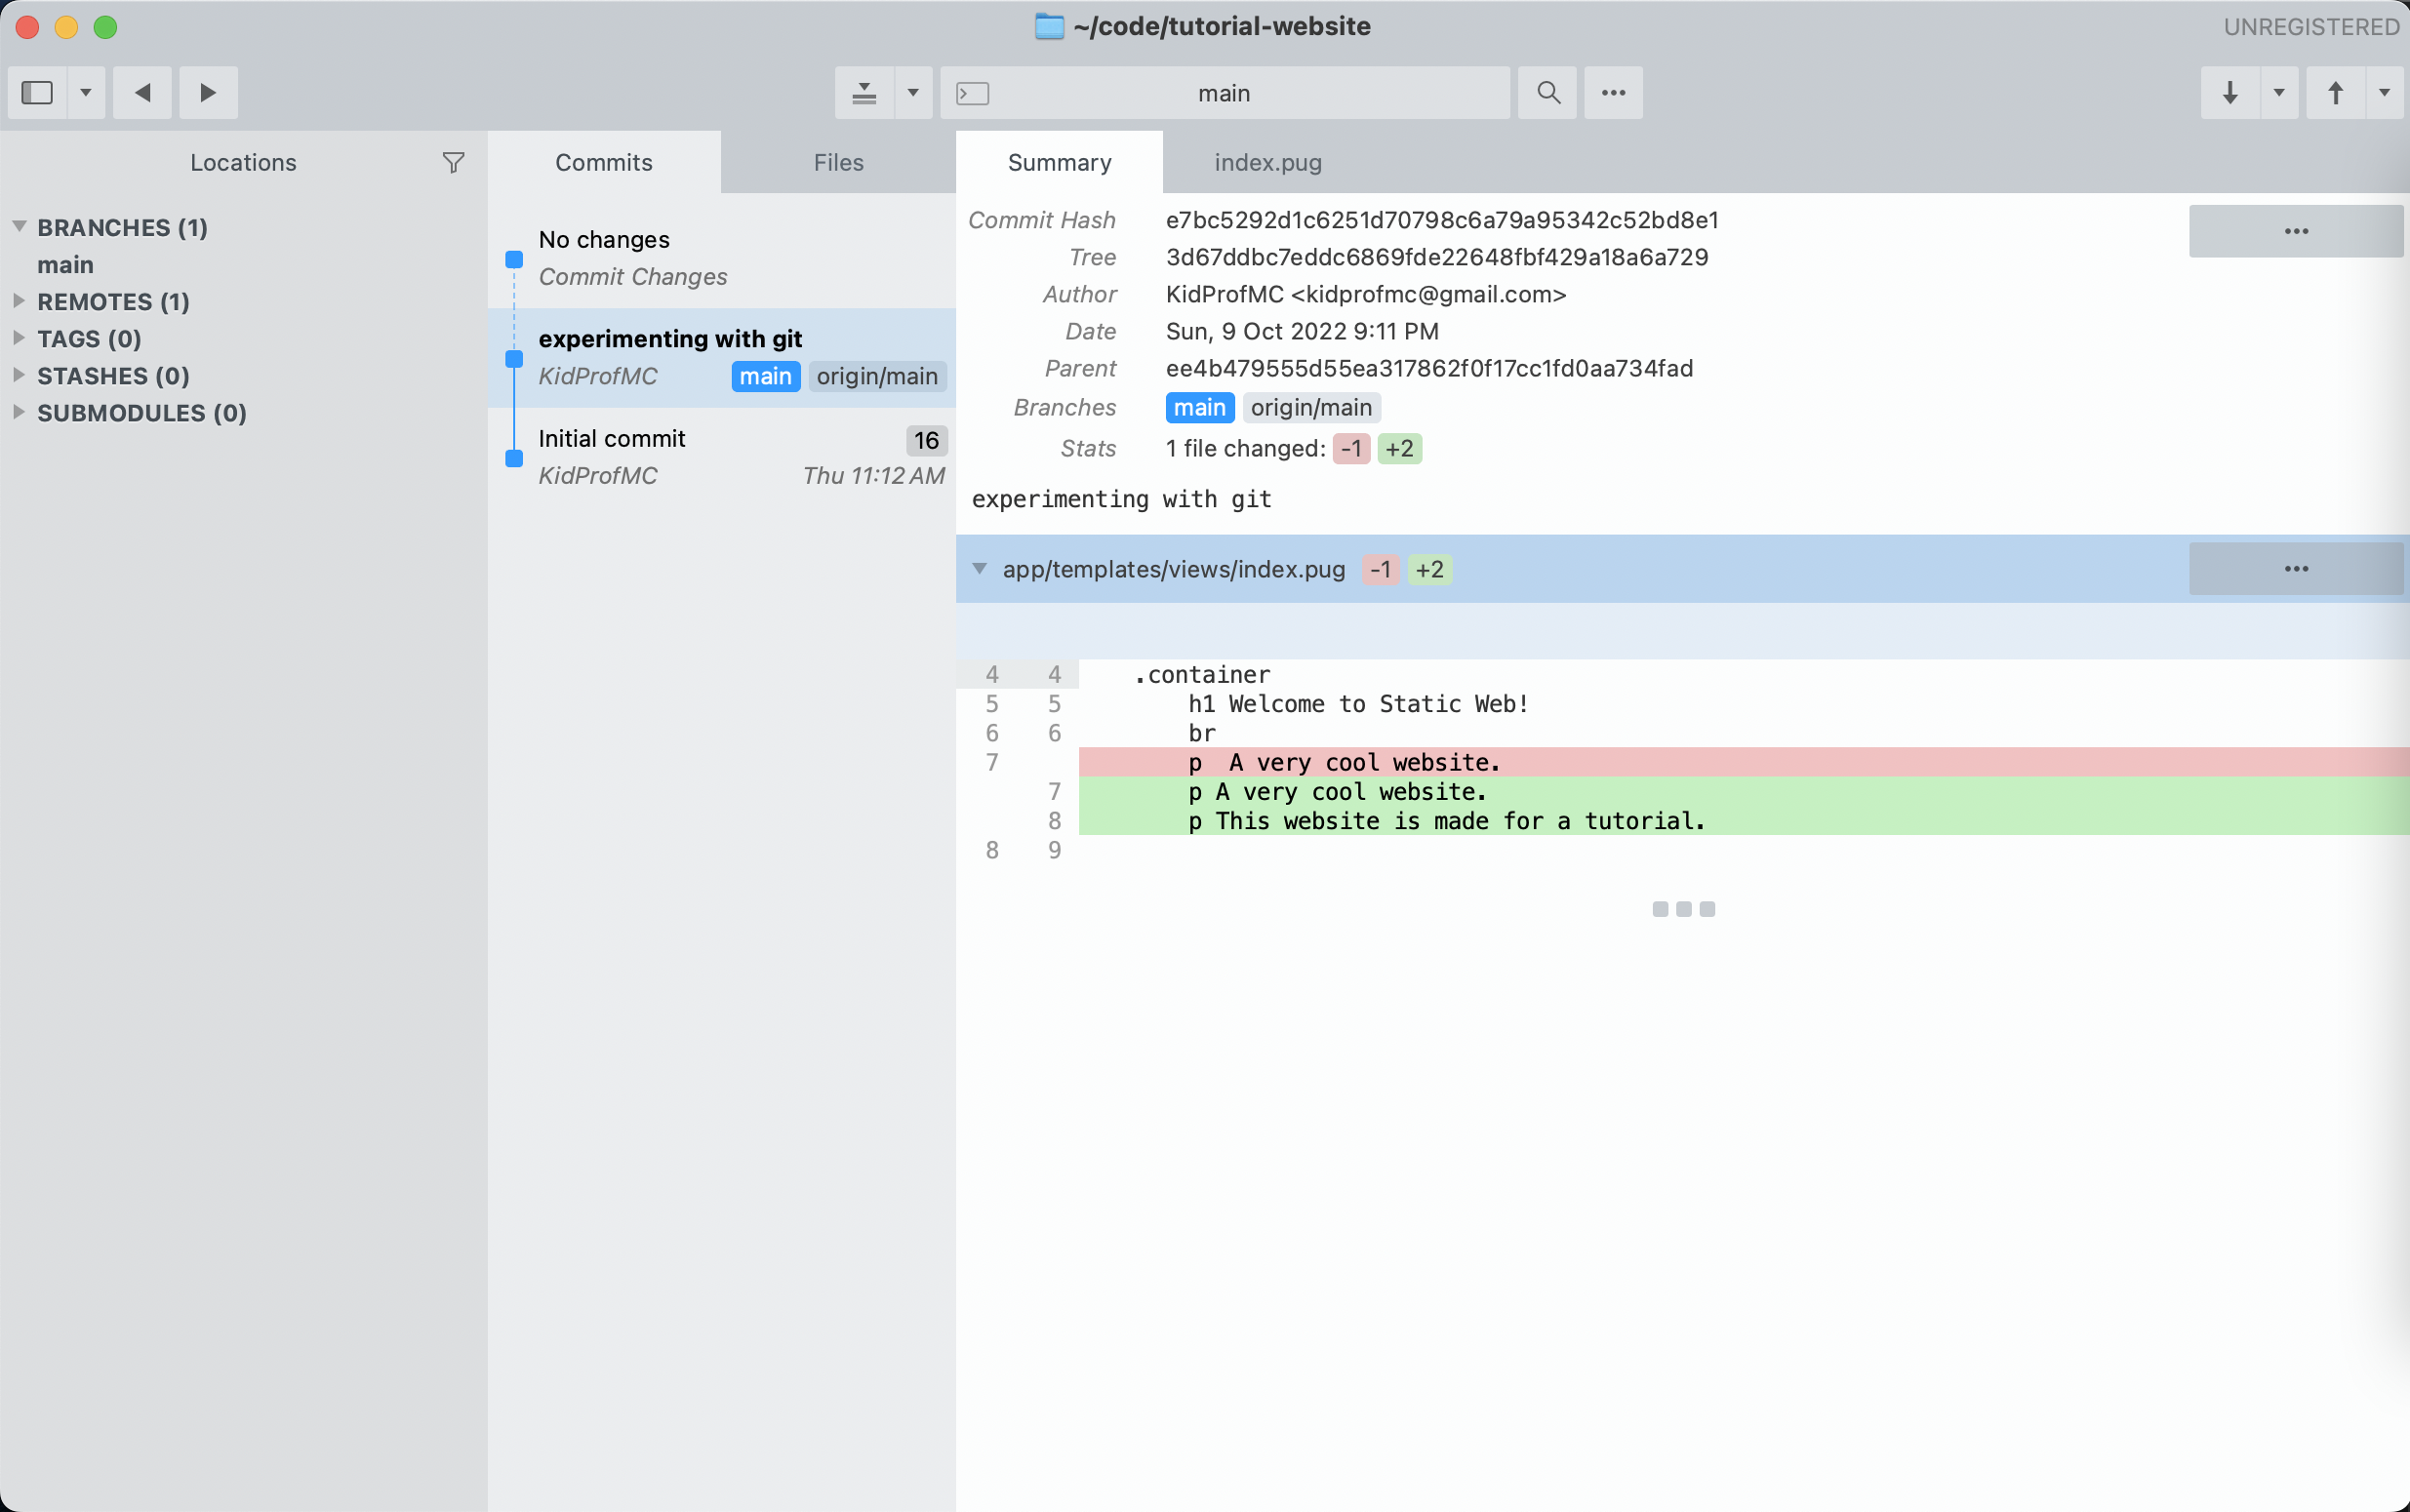
\includegraphics[width=15cm]{images/ch3-sublimemerge.png}
\end{center}

\subsection*{Git Graph}

Git Graph is a VS Code extension, download it inside VS Code.

\begin{center}
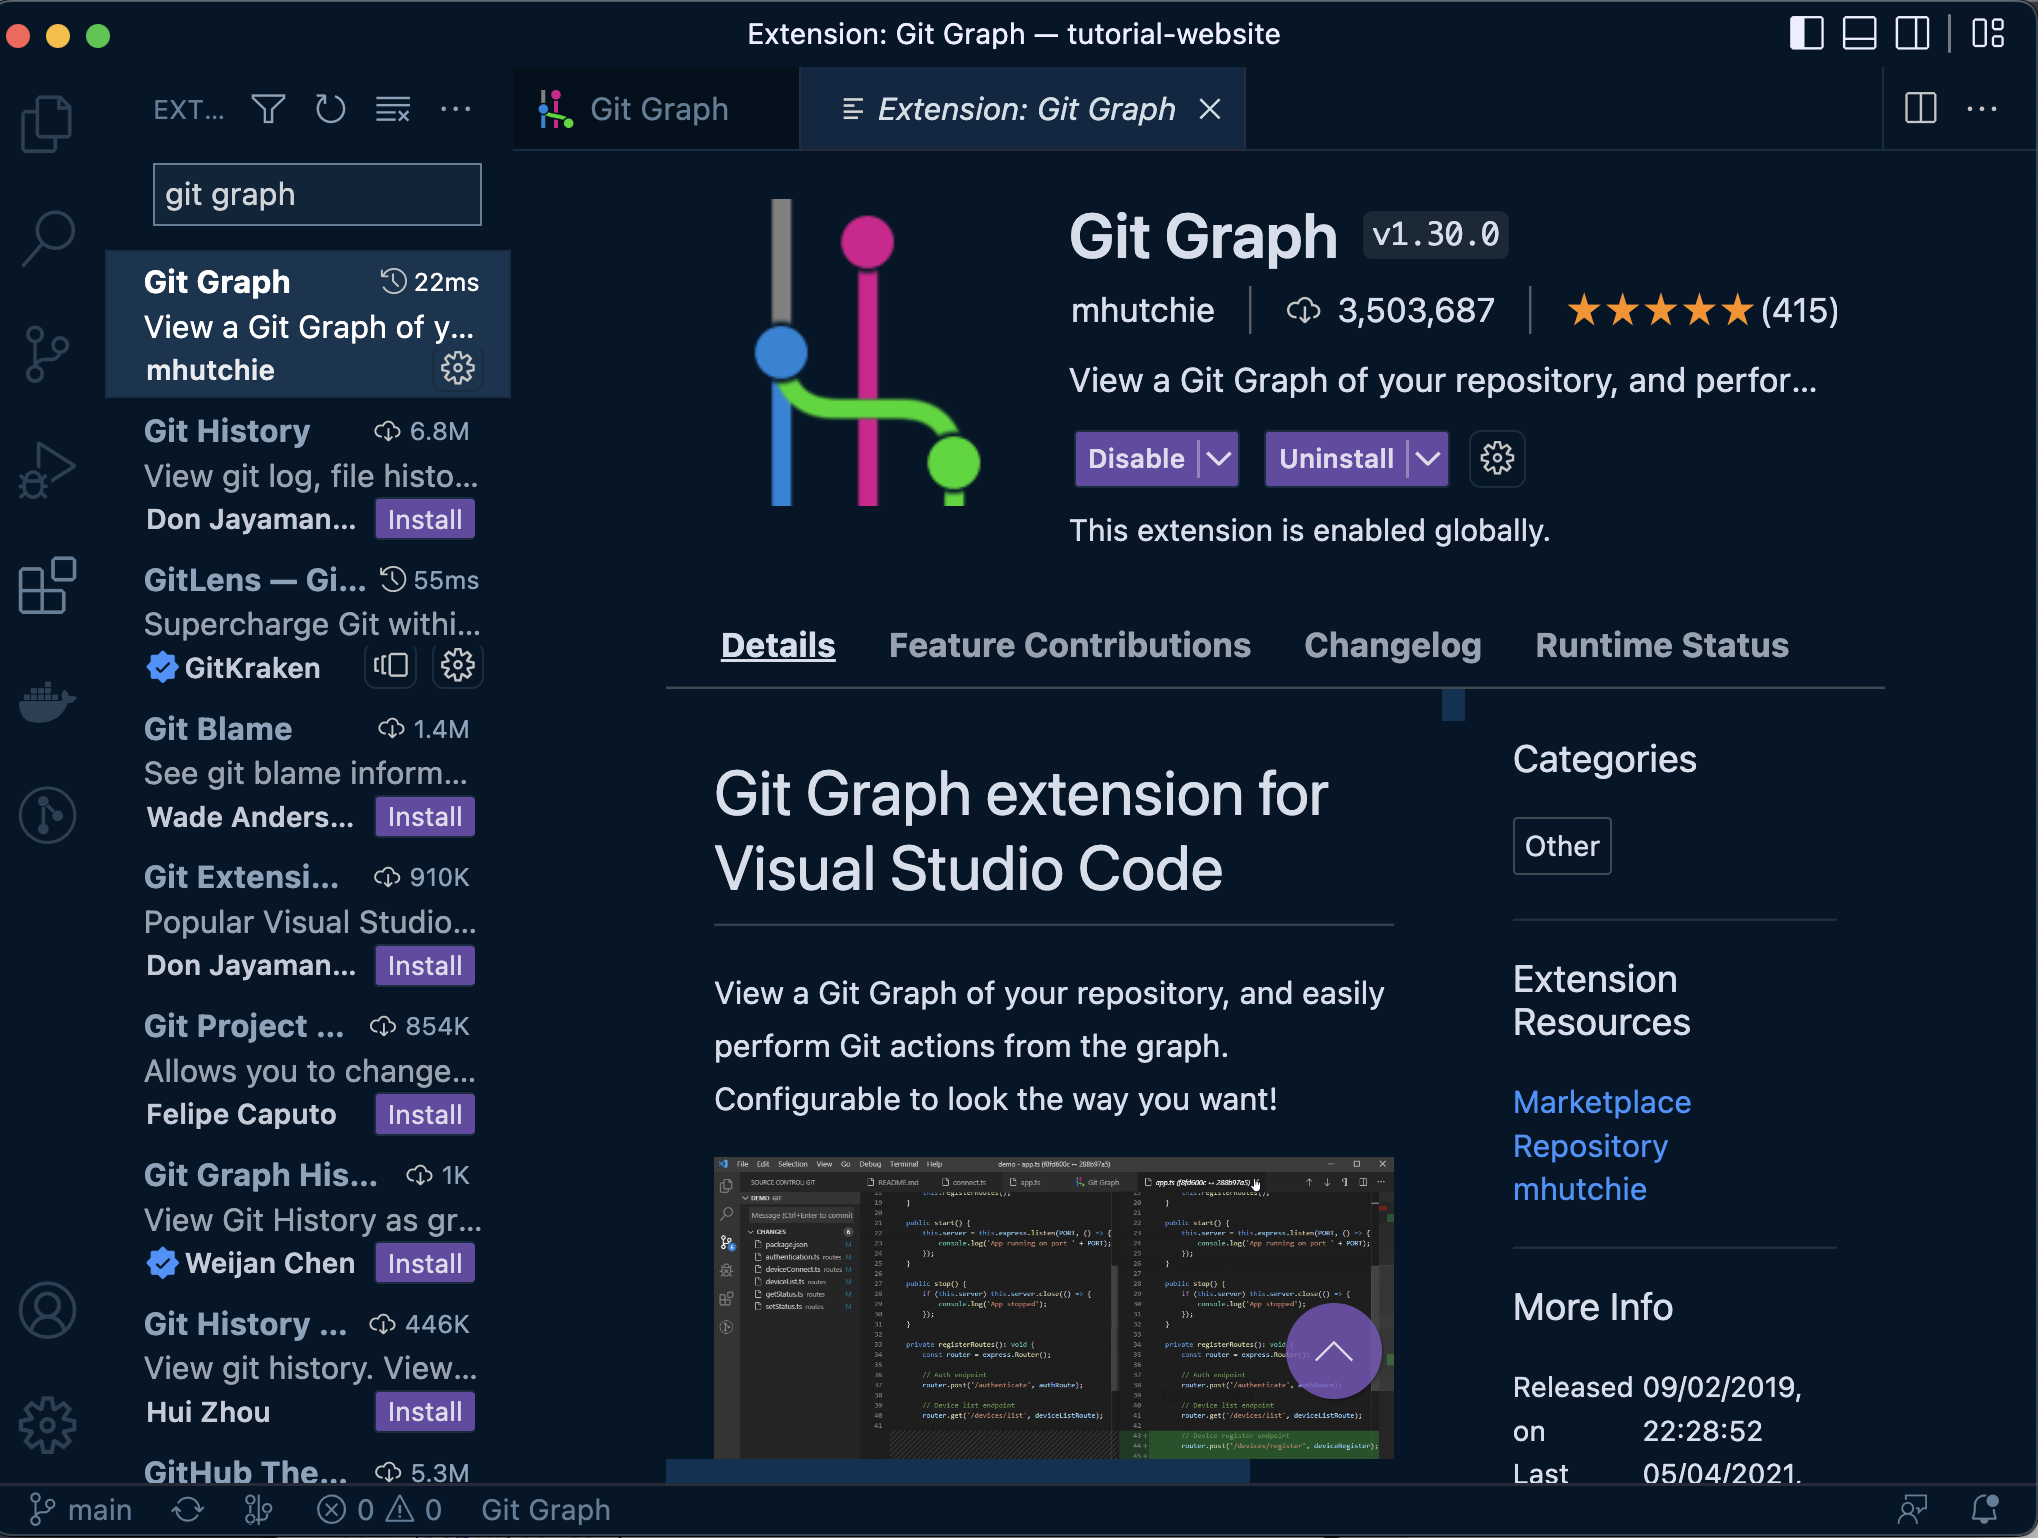
\includegraphics[width=13cm]{images/ch3-gitgraph0.png}
\end{center}

Press \texttt{cmd+shift+P} or \texttt{ctrl+shift+P} to open the VS Code command bar, type \texttt{Git Graph: View Git Graph}

\begin{center}
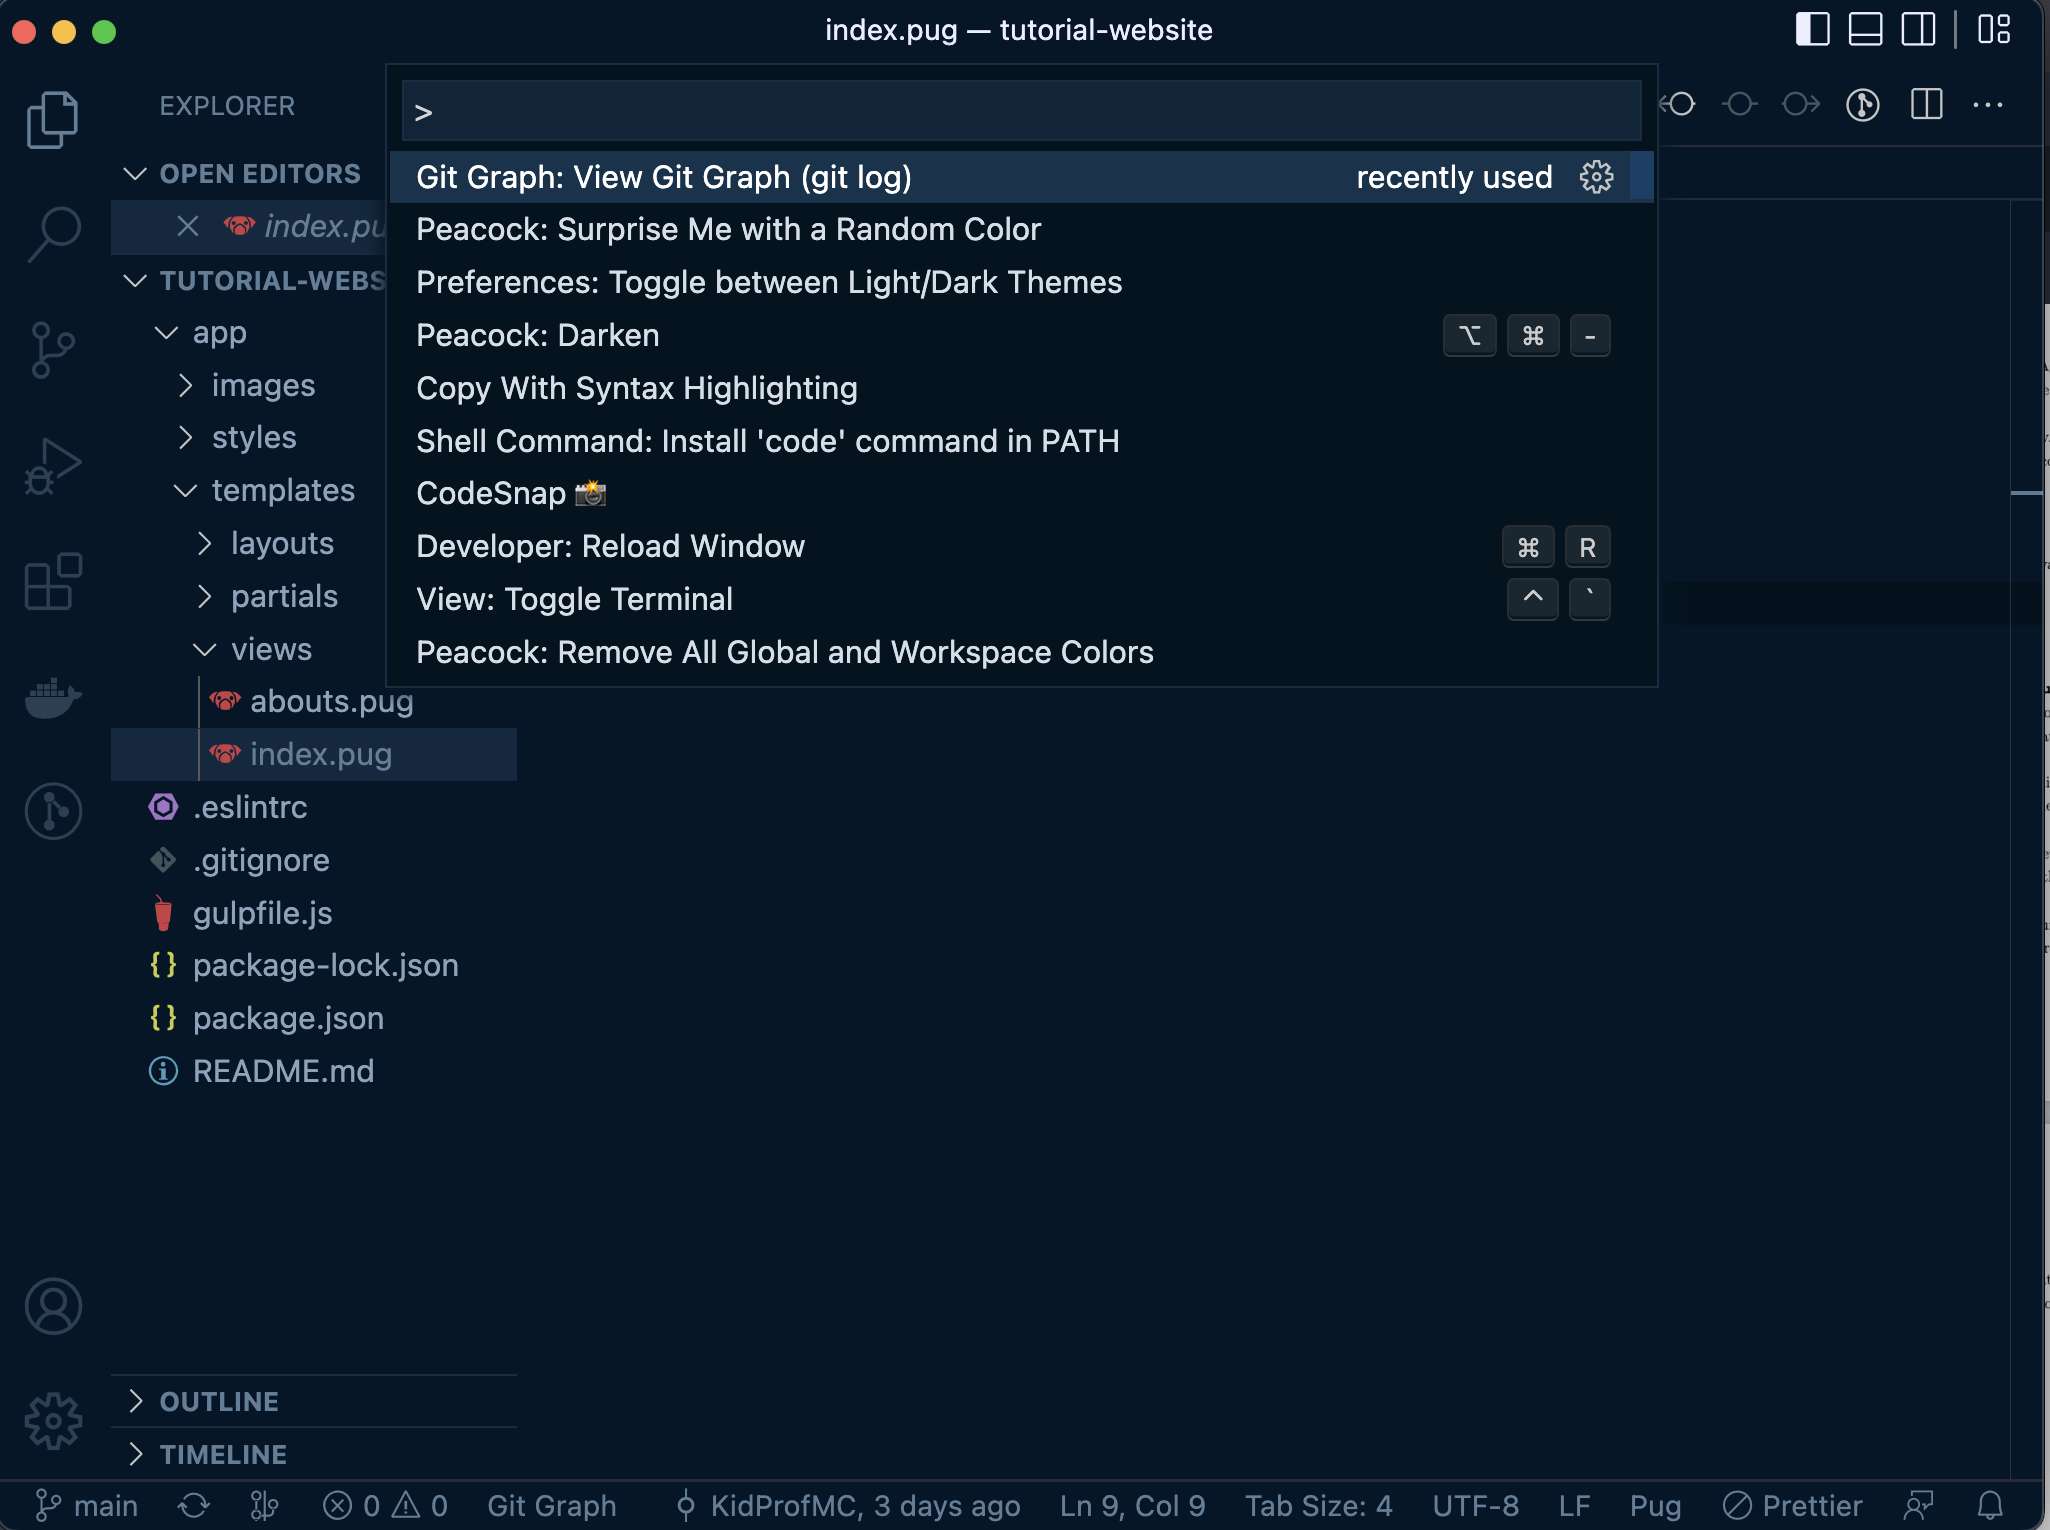
\includegraphics[width=13cm]{images/ch3-gitgraph1.png}
\end{center}

The commit history is displayed.

\begin{center}
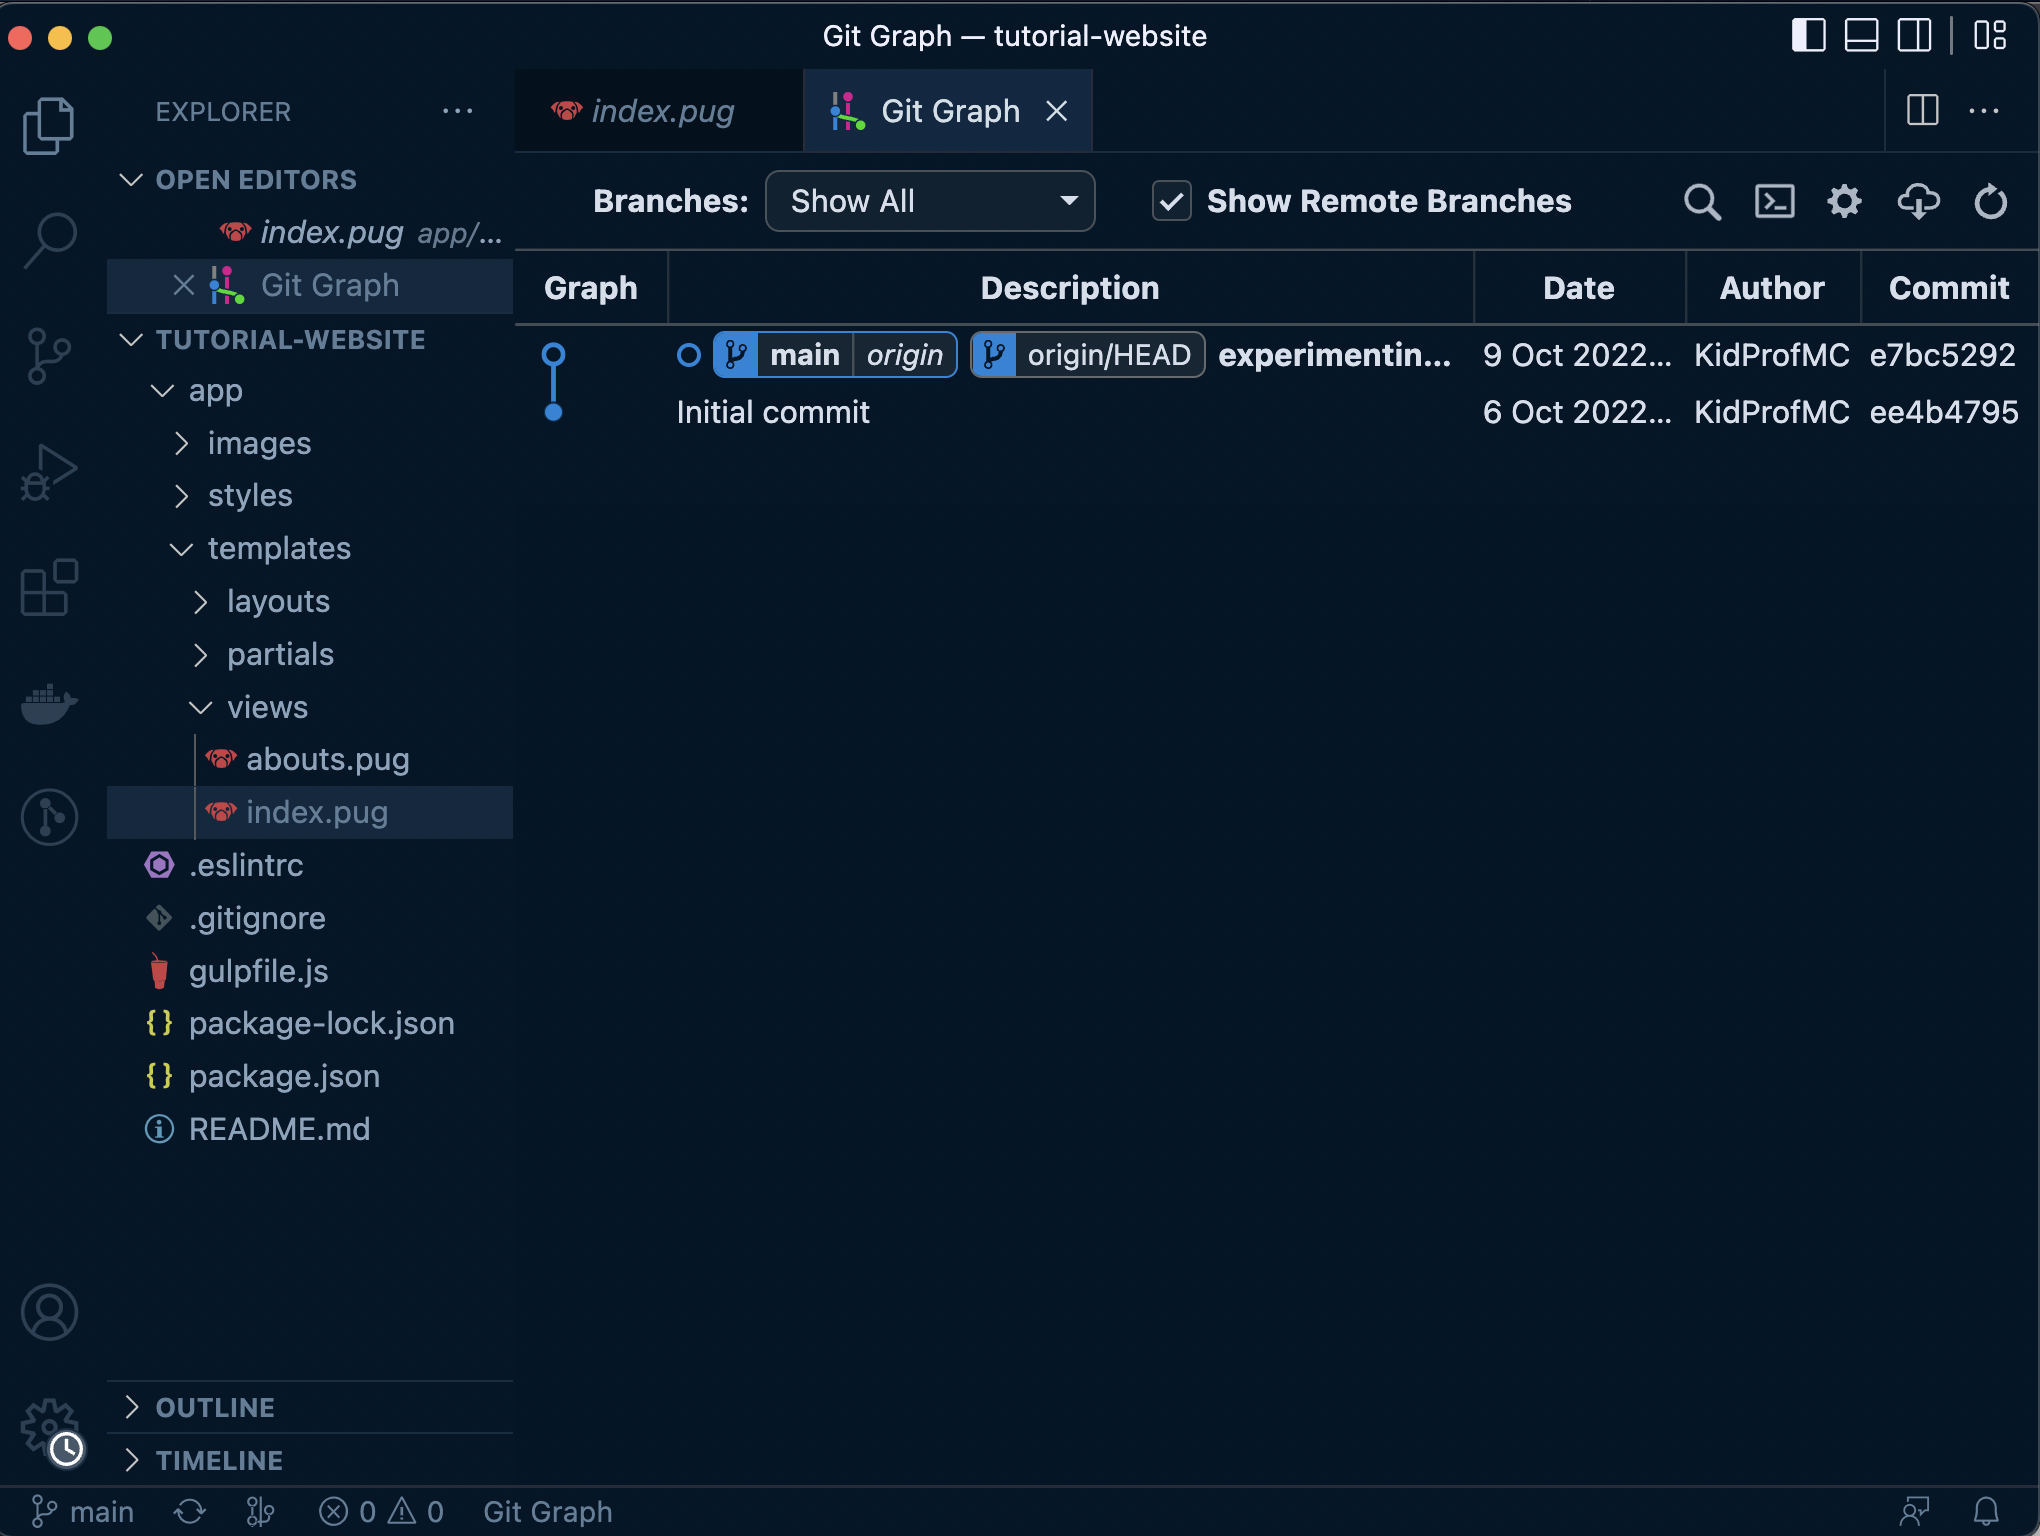
\includegraphics[width=13cm]{images/ch3-gitgraph2.png}
\end{center}

\section{Something went wrong?} 

Anytime if you are unsure about what is happening with Git, \textbf{\texttt{git status}} is your best friend! It will display information about current situation, it might also contains some hints on which command(s) you need to run to get out of nasty situations.
\vspace{6mm}

If you added a files that you don't want to push, and you have not committed, you can try \texttt{git restore <file>} to revert the changes for a particular file, or \texttt{git restore .} to revert all changes.

However, if you made some irreversible/ hard to reverse mistakes, which everybody will at some point in time. For example, you have made a commit at the wrong branch but haven't pushed, or you failed to fix a merge conflict. 

In these cases, let's give up and use a cheesy way to fix it. Move all your code to another location so that you remember what you have changed, clone the repository from GitHub again, then apply your changes to the new copy of the code, but with the mistakes fixed. It is completely fine, and sometimes the easiest way to do something.

\section{Repositories}

\textit{Advanced}
\vspace{6mm}

Again, repository is a fancier name for project. Now we will look closely at this concept, and explain how to establish the relationship between your local code and the GitHub code.

\subsection{Creating a repository on GitHub}
\label{sec:gituploadgithub}

\textit{\textbf{WARNING: } You can only do so when the repository is empty. If the GitHub repository is not empty, you will need to create a new one.}

It is as simple as pressing a "New" button on the GitHub website, then fill in some simple details, such as your repository name and whether you would like your repository to be publicly visible or private, the decision is yours.

You can add a \hyperref[sec:readme]{\texttt{README.md}} or \hyperref[sec:gitignore]{\texttt{.gitignore}}, the usage of such files will be explained in the \hyperref[sec:projstructure]{next chapter}. However, it would make the repository no longer empty and you will have trouble \hyperref[sec:gituploadgithub]{uploading local code to the new repository.}

\subsection{Uploading existing local code to a new GitHub repository}

Use \texttt{git init} in the folder with all your projects.

The use of \texttt{git branch -M main} is to change the name of the default branch from "master" to "main". A decision that GitHub made in 2020.\footnote{More info: \url{https://www.jumpingrivers.com/blog/git-moving-master-to-main/}}

Then follow your normal routine of adding and committing as above in \cref{sec:gcmsg}. There is a convention naming the first commit "init" or "initial commit".

Then \texttt{git remote add origin} is to establish the linkage between the local code and the GitHub repository, so that Git knows where to push to when you run \texttt{git push}, except for the first time, you need to run \texttt{git push -u origin main}.

\begin{lstlisting}[language=bash]
# KidProf in ~/code/your-project
$ git init

# No need to remember, copy from the GitHub docs
$ git branch -M main 

$ git add .
$ git commit -m "init"

# No need to remember, copy from the GitHub docs
$ git remote add origin git@github.com:KidProfMC/git-practice.git
$ git push -u origin main
\end{lstlisting}

\begin{figure}[h]
\centering
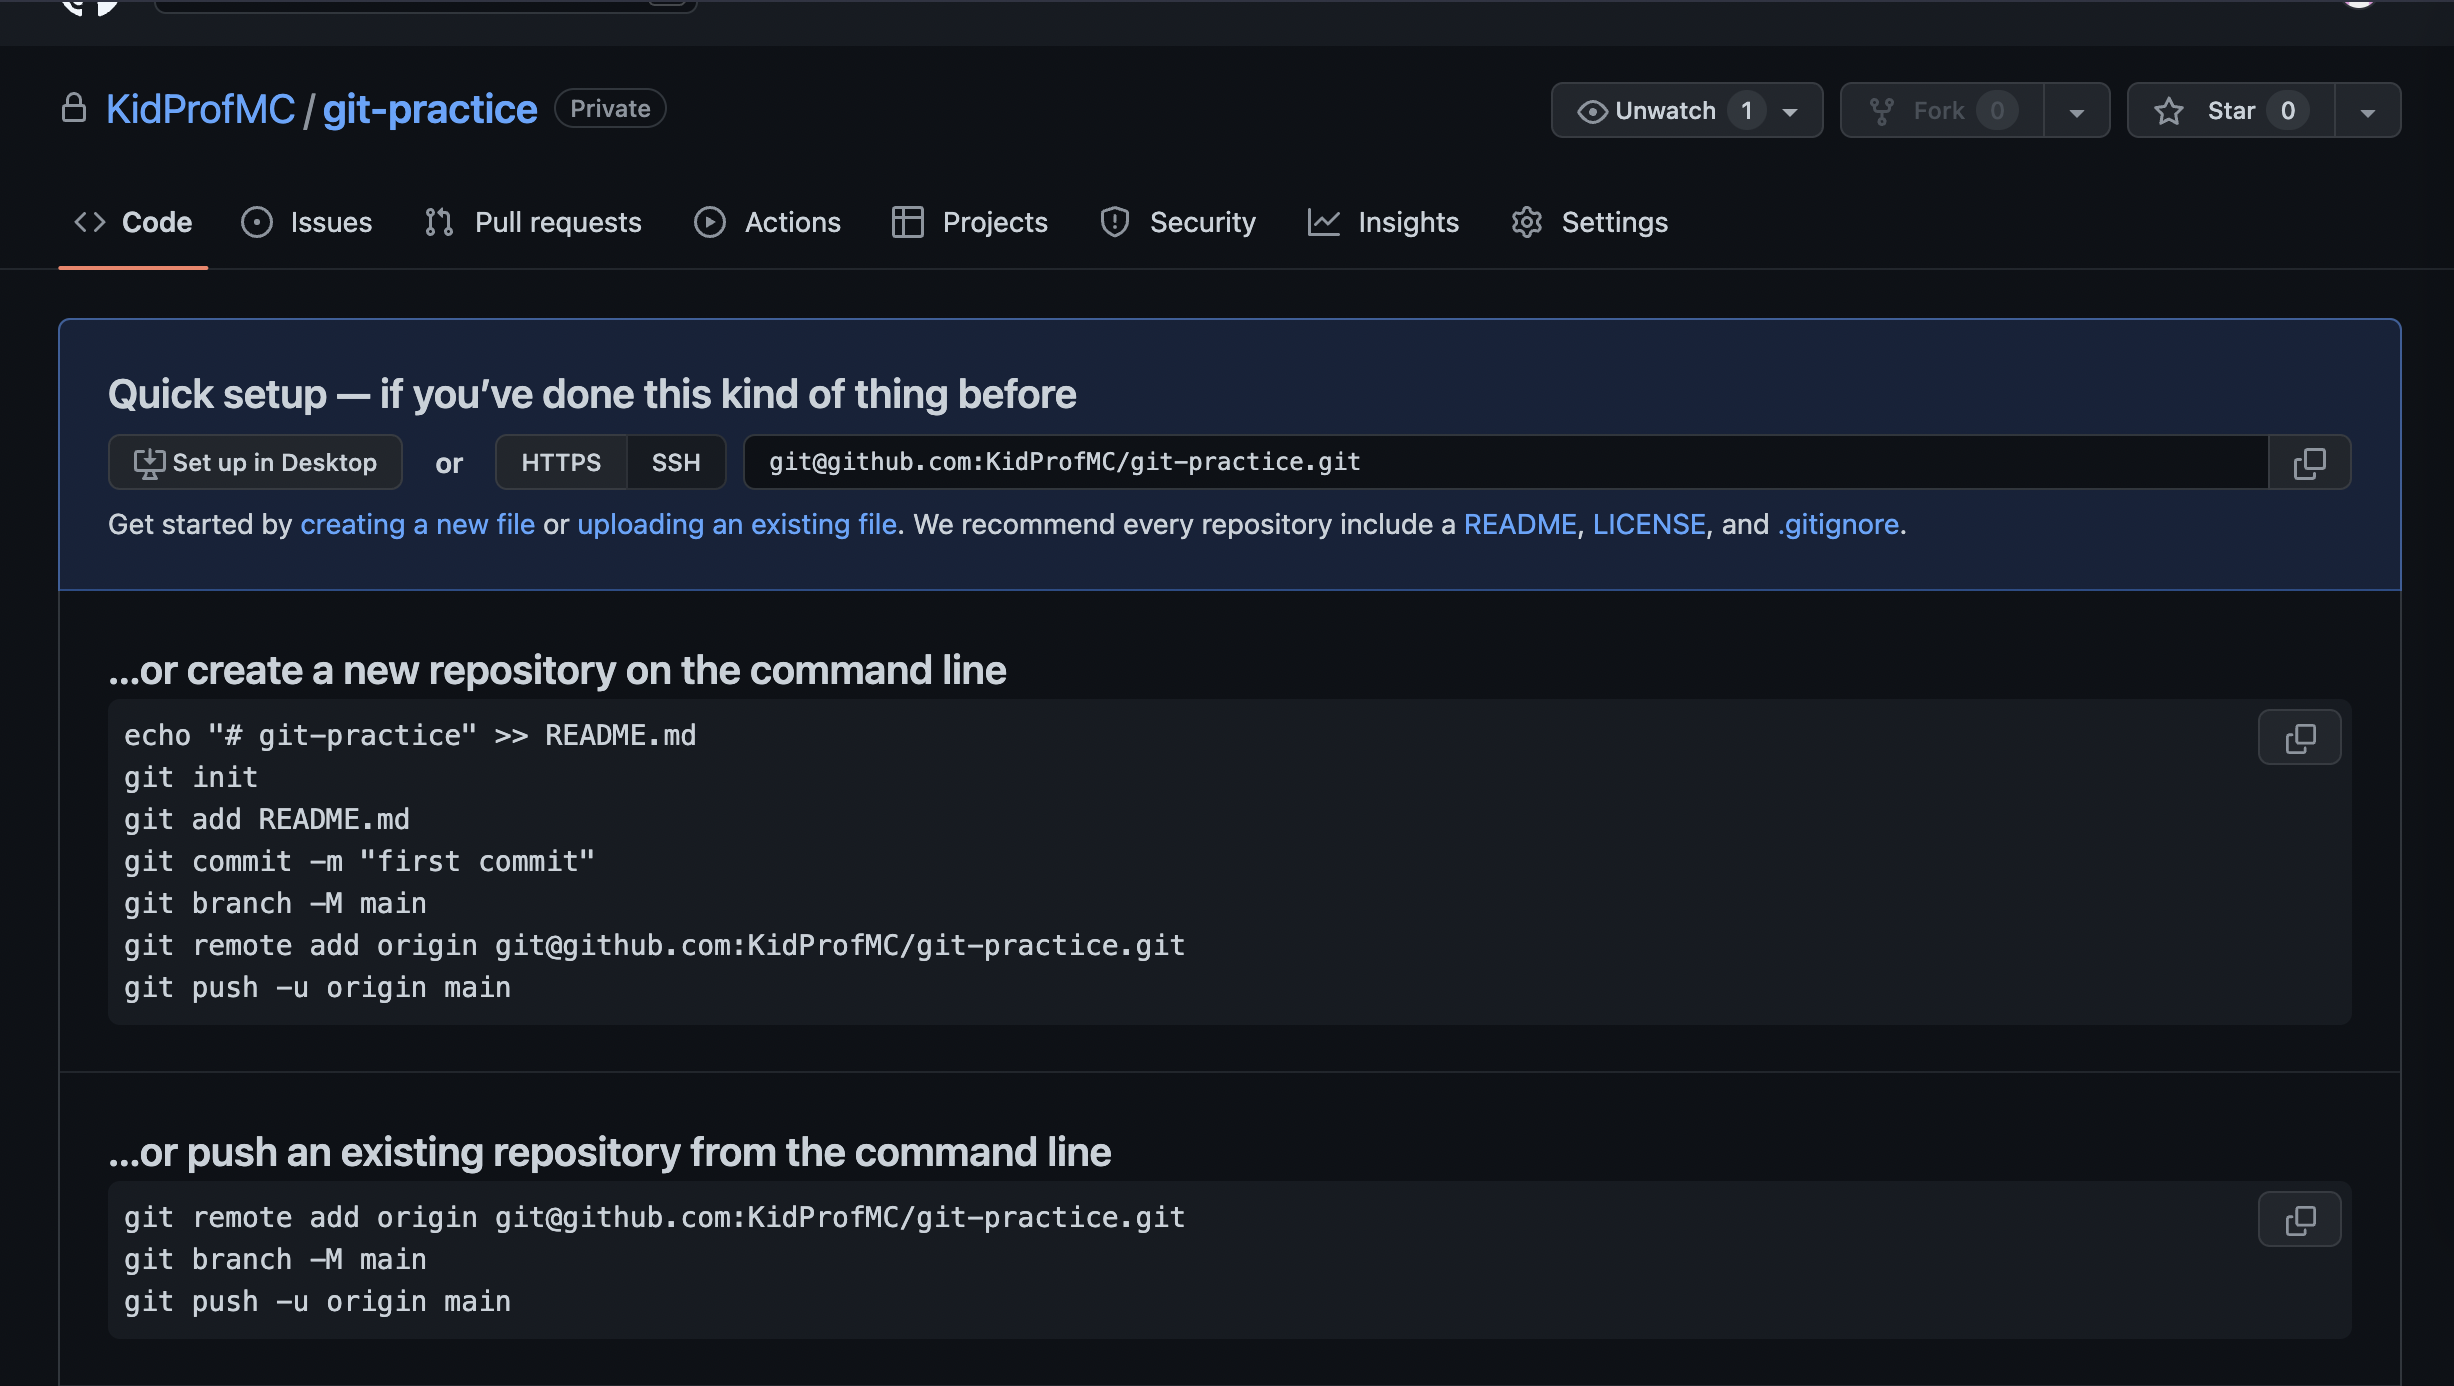
\includegraphics[width=15cm]{images/ch3-newrepocode.png}
\caption{The documentation on GitHub serves you well}
\end{figure}

\subsection{Downloading code from GitHub to local device}
\label{sec:gitclone}

Use \texttt{git clone} followed by the URL provided by GitHub, then a new folder with the repository name would be created with all the code inside. This is the method that we used in \cref{sec:install7}.

\begin{lstlisting}[language=bash]
# KidProf in ~/code
$ git clone git@github.com:KidProfMC/git-practice.git
$ cd git-practice
\end{lstlisting}

\subsection{\texttt{.git} folder}

The \texttt{.git} folder contains everything that git needs to know to function normally, the commit history, the GitHub repository that it is linked to, etc.. If you remove the \texttt{.git} folder from your local device through the file explorer or finder (you need to enable the setting "show hidden files and folders"), or by the command \texttt{rm -rf .git}, all git information would be deleted.


\chapter{Project Structure}
\label{sec:projstructure}

\textit{Covered in \href{https://www.youtube.com/watch?v=fbbjnhs4nyo&list=PLjGmdnqrOKuYXiu7lgG5HW71jPEUd1XCm&index=3}{video 2 of the series}}
\vspace{6mm}

We will tour around the project and explain a little bit on how the website works. It is just a brief overview, you do not need to remember and understand every detail, the most important thing to learn is how to use them, which will be taught in later chapters.

\section{Overview}

The \texttt{app} folder contains everything you need to generate the website. The Pug files, the styles written in Less, JavaScript files, images, etc.. Then by running \texttt{npm run build}, commanding the \texttt{gulpfile.js} and \texttt{node\textunderscore modules} to work together, it translates the Pug files into HTML files, less styles into CSS files, and copies other files to the \texttt{docs} folder. The \texttt{docs} folder is the final output of the website, we can open the HTML files directly using a browser.

\section{Pug files}

Pug files act as template files, we will just call them \textbf{pug files} in this piece of notes. They are translated into HTML files and provide the basic structure of the web page. All Pug files should be put inside \texttt{app/templates}.

\subsection*{Views}

The \texttt{app/templates/views} folder contains the content body of each page. Each Pug file in this folder would be translated to an HTML file with the same name in \texttt{docs}. As you can see, \texttt{abouts.pug} is translated into \texttt{abouts.html} while \texttt{index.pug} is translated into \texttt{index.html}. They all \texttt{extends ../layouts/default}, meaning that they follow the layout in \texttt{app/templates/layouts/default.pug}, which we will look at in a second. (Reminder: \texttt{..} means previous directory)

\texttt{index.pug} (later translated to \texttt{index.html}) is the homepage of the web site. When you host the web page onto a web server, the index page will also be shown when you just type in the URL without specifying which HTML file you want to read. You are advised to have an \texttt{index.pug} file in every project.

\subsection*{Layouts}

The \texttt{app/templates/layouts} folder contains \texttt{default.pug}. It is a template for \textbf{all} pages. It includes common elements like the page title, the styles import, the navbar and the footer. 

Then under \texttt{block content} in line 55, each page in the \texttt{views} folder inserts their own content under this block. Knowing the exact syntax is not required.

\subsection*{Partials}

The navbar and footer are separated from the \texttt{default.pug} to make it cleaner. They are put in the \texttt{app/templates/partials} folder, and got included in \texttt{default.pug} in lines 38 and 61 respectively.

\begin{figure}[h]
\centering
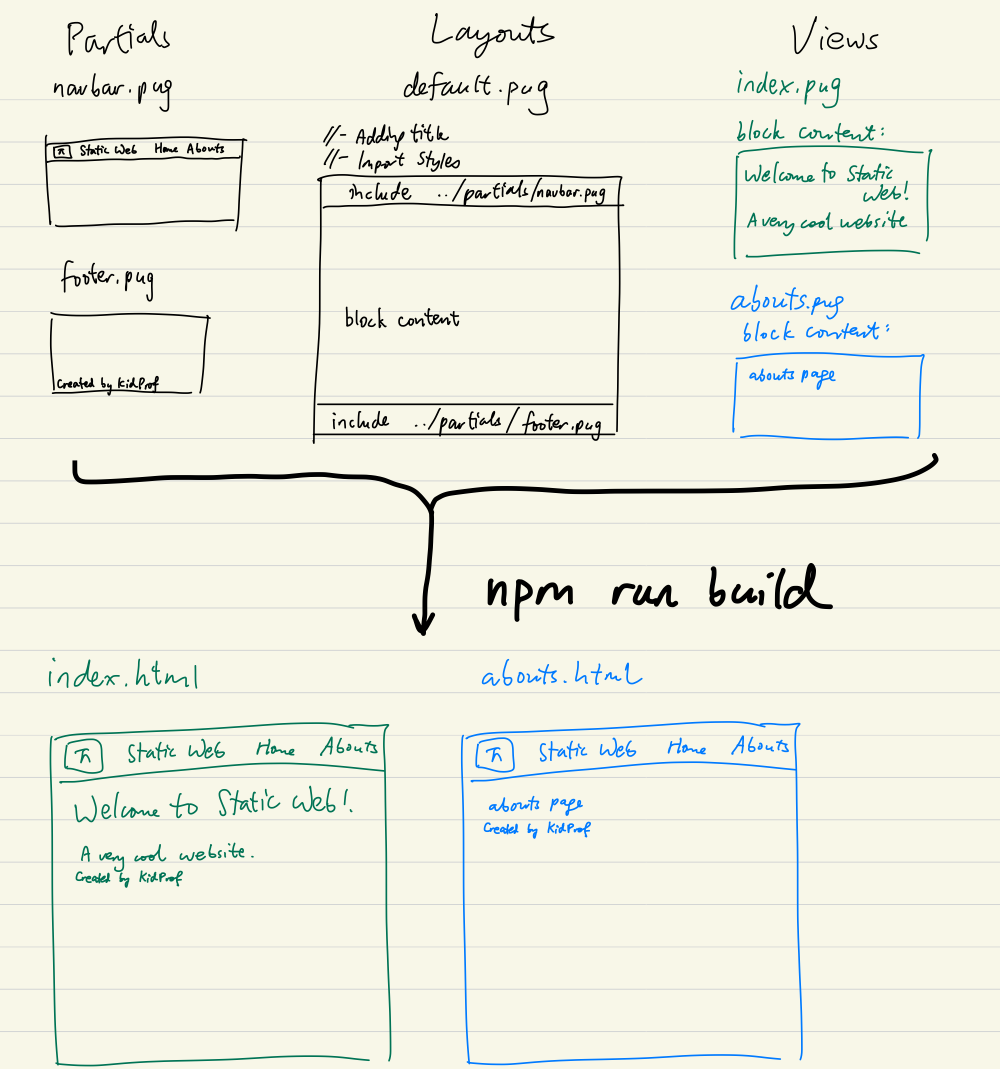
\includegraphics[width=13cm]{images/ch4-puglayouts.png}
\caption{Overview on how Pug files are translated}
\end{figure}

\section{Styling files}

We will be using less files for styling in place for CSS, which are placed under \texttt{app/styles}. We will call them \textbf{Styling files} in this piece of notes. The \texttt{site.less} file includes all files under the \texttt{app/styles/site} folder, \textbf{remember to add the file to \texttt{site.less} whenever you are creating a new less file}. 

The files under the \texttt{site} folder should be where you write the styles. By convention, \texttt{layout.less} should contain styles that is used in all/ multiple pages; \texttt{variables.less} should contain all variables; and other files should contain styles that is only used in the page with the same name as the style file. This is just a convention but not a rule, there is nothing to enforce it until \hyperref[sec:confinestyles]{chapter 8}.

When we run \texttt{npm run build}, the styles got translated into CSS and put into a single file \texttt{docs/styles/site.css}. The stylesheet is imported into all HTML files in line 18 of \texttt{layout.pug}.

\section{Images}

Place all the images or other assets you need for the website under \texttt{\textbf{app}/images} folder. Do not put them inside \texttt{dist}! We will discuss the reasons for that in the next section. 

\section{Website generation}

We kept mentioning \texttt{npm run build} as if it is some sort of magic, now it's time to look a little bit closer.

\subsection{\texttt{package.json}}

This file contains basic information about our project (change the name and description if you like). What is more important is the dependencies and the devDependencies, it tells what \texttt{npm}\footnote{stands for Node Package Manager} what libraries you need to run this project, it is written by me, so all you have to do is to run \texttt{npm install} (what you did already in chapter 1), and it knows what to install for you, without the need of you specifying what to install.

Also the scripts section specifies what will be run on \texttt{npm run ...}, from the line \texttt{"build": "gulp build"}, it means the command \texttt{gulp build} will be run when we run \texttt{npm run build}. More in the \hyperref[sec:gulpfile]{later subsection}.

\begin{lstlisting}[language=]
{
  "name": "static-web-sandbox",
  "version": "2.0.0",
  "description": "A very cool website.",
  "dependencies": {
    "gulp": "^4.0.0"
  },
  "devDependencies": {
    "@babel/core": "^7.2.0",
    "@babel/preset-env": "^7.2.0",
    "gulp-babel": "^8.0.0",
    "gulp-changed": "^3.2.0",
    "gulp-eslint": "^5.0.0",
    "gulp-imagemin": "^5.0.3",
    "gulp-less": "^4.0.1",
    "gulp-pug": "^4.0.1",
    "less-plugin-autoprefix": "^2.0.0"
  },
  "scripts": {
    "test": "echo \"Error: no test specified\" && exit 1",
    "build": "gulp build"
  },
  "license": "ISC"
}
\end{lstlisting}

\subsection{\texttt{node\textunderscore modules} folder}

This folder is automatically generated when you run \texttt{npm install}.\footnote{To verify, remove this folder using \texttt{rm -rf node\textunderscore modules} and run \texttt{npm install} again.} It contains the library files you need to run this project, the project would not run without this folder. \textit{You do not need to edit this file at all.}

\subsection{\texttt{package-lock.json}}

This is an automatically generated file, it outlines in detail which version of the dependencies are installed. It automatically updates when you run \texttt{npm install}. \textit{You do not need to edit this file at all.}

\subsection{\texttt{gulpfile.js}}
\label{sec:gulpfile}

This file is responsible for the translation process. As you can see, the task \texttt{pug} translates each \texttt{.pug} file under \texttt{app/templates/views} to HTML files and put them under \texttt{docs}. Similar translation happens for less files. The JavaScript files, images and fonts are copied to the \texttt{docs} folder.

Finally, the task \texttt{build} runs all the above commands. Therefore, \texttt{gulp build} does what is is supposed to do. \textit{You do not need to edit this file at all.}

\begin{lstlisting}[language=JavaScript]
// gulpfile.js
...

//pug to html conversion
gulp.task('pug', function(){
  return gulp.src("app/templates/views/*.pug")
  .pipe(changed("docs/")) //pipe files only if changed 
  .pipe(pug({pretty:true})) //pug to html
  .pipe(gulp.dest('docs/'));
});

//less to css conversion
gulp.task('styling', function(){
  return gulp.src("app/styles/site.less")
  .pipe(changed("docs/styles")) //pipe files only if changed 
  .pipe(less({
    plugins: [autoprefix]
  })) //less to css
  .pipe(gulp.dest('docs/styles'));
});

gulp.task('js',function(){ ... });
gulp.task('imagecopy',function(){ ... });
gulp.task('fontcopy',function(){ ... });

gulp.task('build',gulp.series('js','pug','styling','imagecopy','fontcopy'));

\end{lstlisting}

\subsection{\texttt{docs} folder}

This folder is automatically generated when you run \texttt{run build}.\footnote{To verify, remove this folder using \texttt{rm -rf docs} and run \texttt{npm run build} again.} It is the output folder of the whole project, you can directly open the HTML files inside the folder. You should upload this folder to web servers in order to host it.
\textit{You do not need to edit this file at all.}
\vspace{6mm}

\textbf{IMPORTANT: Do NOT edit anything in the \texttt{docs} folder. Changes will be overwritten when you run \texttt{npm run build} again.}

\subsection{\texttt{.gitignore}}
\label{sec:gitignore}

Because the \texttt{node\textunderscore modules} folder and the \texttt{docs} folder can be automatically generated on your own local machine. There is no need to put these onto GitHub. The \texttt{.gitignore} file lets you state the files and folders that you do not want to push to GitHub. It includes the two folders I have mentioned, and some others that are out of our scope.

\section{Other files}

\subsection{\texttt{README.md}}
\label{sec:readme}

This file serves as a documentation. It will be displayed on GitHub. You should write a description of your project, and how to install and use it in here. The syntax is a bit weird, refer \href{https://docs.github.com/en/get-started/writing-on-github/getting-started-with-writing-and-formatting-on-github/basic-writing-and-formatting-syntax}{here}\footnote{Link: \url{https://docs.github.com/en/get-started/writing-on-github/getting-started-with-writing-and-formatting-on-github/basic-writing-and-formatting-syntax}} if you want to write your own README.

\subsection{\texttt{.eslintrc}}

\textit{Of less importance}
\vspace{6mm}
This file stores the JavaScript settings and version we are using, so as to check for syntax errors when copying JavaScript files from \texttt{app} to \texttt{docs}. \textit{You do not need to edit this file at all.}

\section{VS Code Tips}

You can run \texttt{code .} in your terminal to open VS Code with the directory opened, it is very convenient. If you can't get it to work, try setting up the environment variables as instructed \href{https://code.visualstudio.com/docs/setup/mac}{here}\footnote{Link: \url{https://code.visualstudio.com/docs/setup/mac}}.
\vspace{6mm}

Another good tip is that you can highlight a few lines of text, and hit \texttt{tab}, and all those lines will be indented inwards; while hitting \texttt{shift+tab} will make them indent outwards.
\vspace{6mm}

As I have said before, it is not a must to install any plugins.
\chapter{Pug.js}

Pug.js (abbreviated as Pug) files are translated into HTML files, they provide the basic structure of the web page. Now let's learn how to write our own web page using Pug.

\section{Further Resources (Ch 5)}

I didn't have this piece of notes back when I first learned Pug. Here is \href{https://youtu.be/kt3cEjjkCZA}{the video}\footnote{Link: \url{https://youtu.be/kt3cEjjkCZA}{the video}} that I used to learn the basics. 

You could refer to the \href{https://www.w3schools.com/tags/default.asp}{w3schools documentation}\footnote{Link: \url{https://www.w3schools.com/tags/default.asp}} to learn how to use some more HTML tags.

\section{Magic on the Pug.js website}

The \href{{https://pugjs.org/}}{Pug.js official website}\footnote{Link: \url{https://pugjs.org/}} contains a detailed documentation on how it is translated to HTML.

What's more valuable is its interactive translator, you can just type any Pug code on any page in the documentation, \href{https://pugjs.org/language/attributes.html}{like this one}\footnote{Link: \url{https://pugjs.org/language/attributes.html}}, type Pug code on the left box and it will translate to HTML code on the right. It is a very useful tool to experiment with the Pug language.

\begin{figure}[h]
\centering
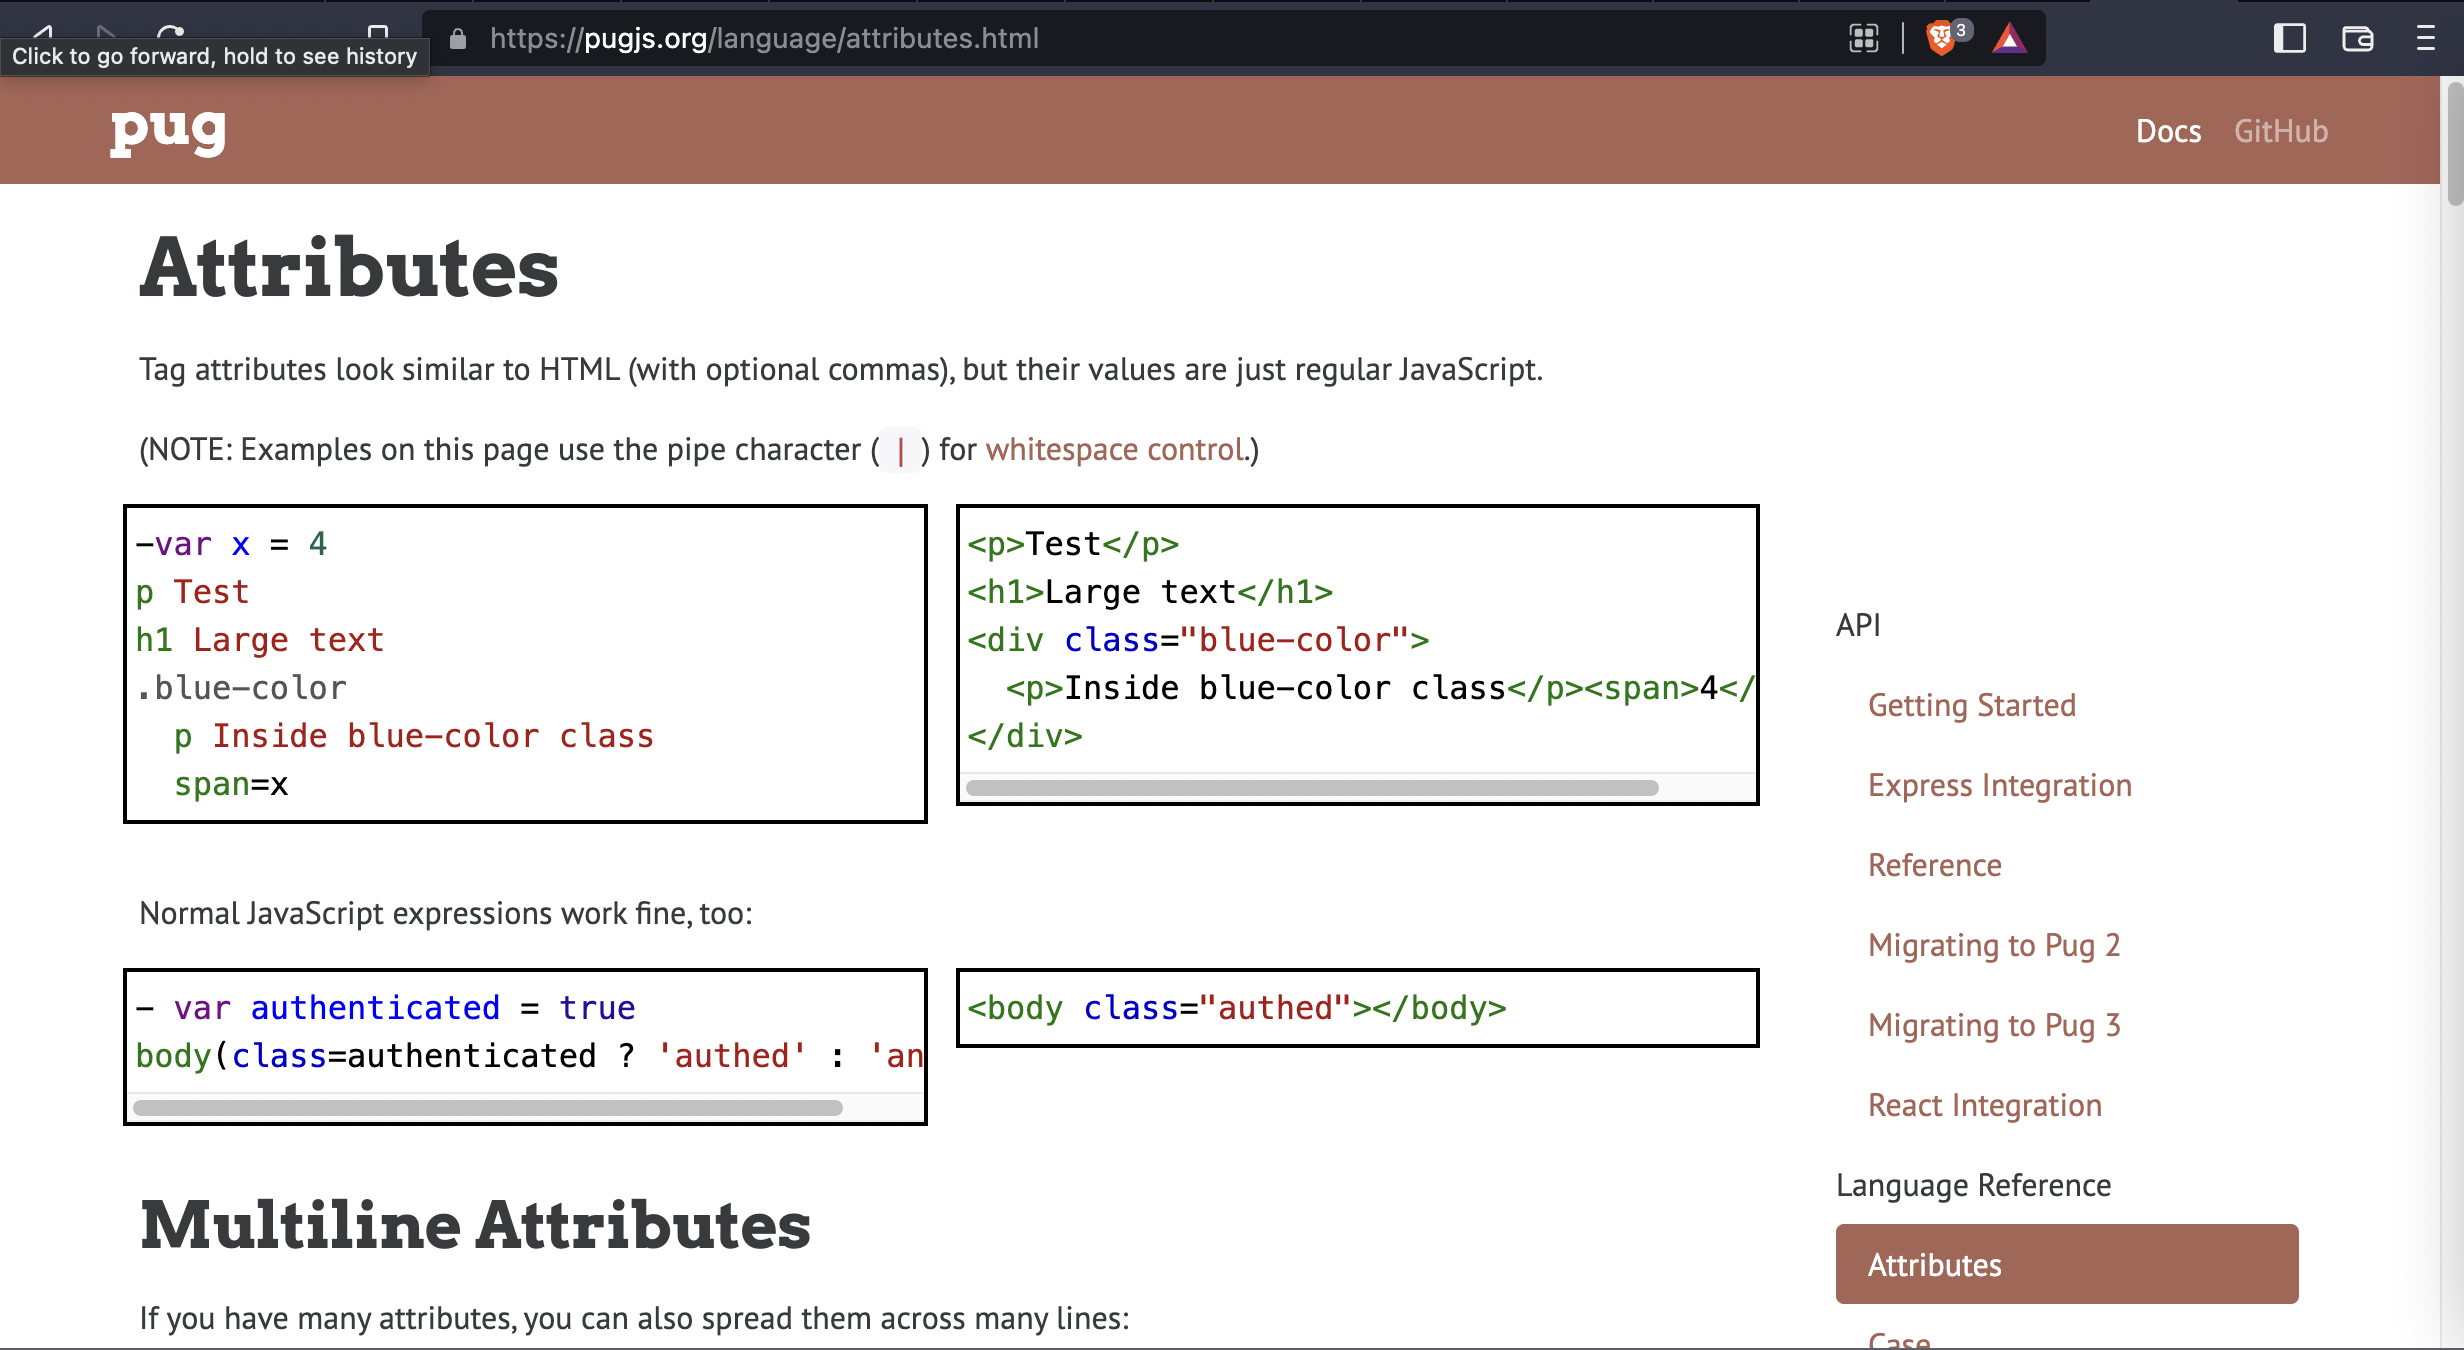
\includegraphics[width=13cm]{images/ch5-puginteractive.png}
\caption{Example usage of the interactive translator on the Pug.js official website}
\end{figure}

\section{HTML Tags}

Some of you haven't coded in HTML before, so here is a quick walkthrough to the basics of HTML, but using Pug.js syntax. For those of you who have used HTML before, mind the syntactical difference, a summary of the differences will be provided in one of the \hyperref[sec:pugvshtml]{sections below}. You can experiment the output in any file under \texttt{app/templates/views}, under the \texttt{block content} section.

\subsection{Normal text}

\texttt{p} stands for paragraph. Use this for normal text.
\vspace{6mm}

\begin{lstlisting}[language=pug]
p Hello world
\end{lstlisting}

\subsection{Headers}

\texttt{h1} stands for header 1, \texttt{h2} stands for header 2, and so on until \texttt{h6}. With \texttt{h1} being the largest. Use this for titles and subheadings.
\vspace{6mm}

\begin{lstlisting}[language=pug]
h1 header 1
h2 header 2
h3 header 3
h4 header 4
h5 header 5
h6 header 6
\end{lstlisting}

\subsection{Images}

\texttt{img} stands for image. You need to specify the source \texttt{src} of the image using \textbf{attributes}, we surround the attributes in parenthesis in Pug. Please make sure you add your images in the \texttt{app/images} folder.
\vspace{6mm}

\begin{lstlisting}[language=pug]
img(src="images/pi-green.png")
\end{lstlisting}

You can specify its width and height in pixels.

\begin{lstlisting}[language=pug]
img(src="images/pi-green.png" width=100 height=100)
\end{lstlisting}

\subsection{Links}

Use the \texttt{a} tag for links. It requires an \texttt{href} attribute indicating where the link should go.
\vspace{6mm}

\begin{lstlisting}[language=pug]
a(href="abouts.html") Click to go to the abouts page.
\end{lstlisting}

To open a brand new tab instead of replacing the current one, add the attribute \texttt{target = "\textunderscore blank"}
\vspace{6mm}

\begin{lstlisting}[language=pug]
a(href="https://www.google.com" target="_blank") Click to open Google on a new tab.
\end{lstlisting}

\subsection{Lists}

We surround all contents of a list within a \texttt{ul} or a \texttt{ol} tag. We use \texttt{ul} (unordered list) when we need bullet points, while we use \texttt{ol} (ordered list) when we need numbering. Each bullet point is demoted by \texttt{li} (list element).

The "surrounding" I mentioned is achieved by indenting all \texttt{li} tags within the \texttt{ul} or \texttt{ol} tags.
\vspace{6mm}

\begin{lstlisting}[language=pug]
ul
    li Apples
    li Oranges
    li Pears

p When you got an error message you should:
ol
    li Copy the error message
    li Go to <a href="https://www.google.com"> Google</a>
    //- The syntax used for the a tag will be discussed in the br tag section.
    li Paste and search for the error message
    li Click on the first stack overflow result
    li Copy and paste the solution
\end{lstlisting}

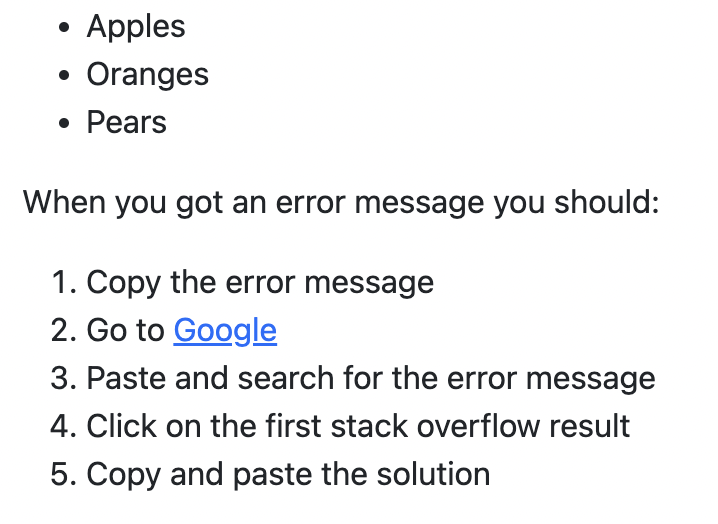
\includegraphics[width=10cm]{images/ch5-ulol.png}

\subsection{\texttt{div}}

\texttt{div} stands for divider. It serves no purposes in adding content to the web page, but it can be used to improve organisation of your code, and it is crucial for styling. We will discuss more in the \hyperref[sec:classesids]{next section} and also in the \hyperref[sec:ch6]{next chapter}.
\vspace{6mm}

\begin{lstlisting}[language=pug]
div
    h1 Self introduction
    p ...
div
    h1 Contact methods
    ul
        li ...
        ...
\end{lstlisting}

\subsection{\texttt{br}}

When the text is too long, you can put a \texttt{.} after the tag, and it now regards what indented within the tag as text.

\begin{lstlisting}[language=pug]
p.
    Hello, I am KidProf.
    I am a university student studying Computer Science.
    I like coding.
\end{lstlisting}


\includegraphics[width=15cm]{images/ch5-textinaline.png}

But when you look at the output, they are all on the same line. This is because the line breaks you made in the code is independent of the line breaks shown on the web page, you need to explicitly use \texttt{br} tags for line breaks. Because we are inside the \texttt{p} tag, Pug regards everything inside as text but not tags, but we can still use conventional HTML syntax to get around it.

\begin{lstlisting}[language=pug]
p.
	Hello, I am KidProf. <br />
	I am a university student studying <br />Computer Science.<br />
	I like coding.
\end{lstlisting}


\includegraphics[width=15cm]{images/ch5-textmultiplelines.png}

Alternatively, if you do not like that normal HTML code in your Pug code, you could do this instead and lead to the same result. But this is a lot of effort and affects code readability.

\begin{lstlisting}[language=pug]
p
	| Hello, I am KidProf.
	br
	| I am a university student studying
	br
	| Computer Science.
	br
	| I like coding.
\end{lstlisting}

The removal of the \texttt{.} after \texttt{p} indicates that what indented within are tags instead of plain text, so the \texttt{br} tags are registered. To indicate that the rest are plain text, the \texttt{|} character is used.

\subsection{Comments}

Use \texttt{//-} for comments.\footnote{An alternative is \texttt{//}, using \texttt{//} means that the generated HTML file would also contain that comment, while using \texttt{//-} won't.}

\subsection{I am lazy}
There are also other useful HTML tags, like \texttt{table}, \texttt{tr}, \texttt{td}, \texttt{span}, \texttt{small}, \texttt{button}, \texttt{input}. You could refer to the \href{https://www.w3schools.com/tags/default.asp}{w3schools documentation}\footnote{Link: \url{https://www.w3schools.com/tags/default.asp}} to learn how to use these tags. The translation to Pug is similar to the tags mentioned above.

\section{Classes and IDs}
\label{sec:classesids}

We need the notion of classes and IDs to do styling in the \hyperref[sec:ch6]{next chapter}, so that we can reference elements that we would like to style from the styling files.

We use \texttt{\#} followed by text to indicate an ID, and we use \texttt{.} followed by text to indicate a class. ID and class names must not contain spaces, it is a convention to either use camelCase or hyphens in place of spaces.
\vspace{6mm}

\begin{lstlisting}[language=pug]
div#self-intro
	h1 Self introduction
	p.large-text.
		Hello, I am KidProf. <br />
		I am a university student studying <br />Computer Science.<br />
		I like coding.
ul#shopping-list
	li Apples
	li.warning Oranges
	li.warning Pears
p When you got an error message you should:
ol#error-list
	li Copy the error message
	li Go to <a href="https://www.google.com"> Google</a>
	li Paste and search for the error message
	li Click on the first stack overflow result
	li Copy and paste the solution
a(href="#self-intro") Back to top
\end{lstlisting}

In the code above we have defined a few IDs, including \texttt{\#self-intro}, \texttt{\#shopping-list}, \texttt{\#error-list}; and also a few classes, including \texttt{.warning} and \texttt{.large-text}. 
\vspace{6mm}

\textbf{IDs must be unique within a page, while there can be multiple elements with the same class name in the same page.} An element can have more than one class.
\vspace{6mm}

To demonstrate one of the uses of IDs, I have included a link at the bottom of the example code. When you click on it, it brings you to the start of the page, to the element with ID \texttt{self-intro}. This feature does not work for classes because multiple elements can have the same class name in the same page.

The use of classes and IDs would become clearer in the \hyperref[sec:ch6]{next chapter}.

\section{Pug VS HTML syntax}
\label{sec:pugvshtml}

\textit{Skip if you have not learnt HTML before, this section aims to allow HTML programmers to relate what we are learning to what they have learnt}
\vspace{6mm}

Pug uses indentation to indicate that something is in a tag while HTML uses closing tags.
\vspace{6mm}

\begin{lstlisting}[language=pug]
//- pug
ul
  li A
  li B
  li C
\end{lstlisting}

\begin{lstlisting}[language=html]
<!-- HTML - poorly formatted, but would still work! -->
<ul><li>A</li><li>B</li><li>C</li></ul>
\end{lstlisting}

All attributes should be put within parenthesis after the tag in Pug, while attributes should be put within the opening tag in HTML.
\vspace{6mm}

\begin{lstlisting}[language=pug]
//- pug
a(href="abouts.html") Click to go to the abouts page.
\end{lstlisting}

\begin{lstlisting}[language=html]
<!-- HTML -->
<a href="abouts.html">Click to go to the abouts page.</a>
\end{lstlisting}

Classes and IDs declarations can be simplified with Pug using the syntax shown in the \hyperref[sec:classesids]{last section}.
\vspace{6mm}

\begin{lstlisting}[language=pug]
//- pug
a#abouts-link.class1.class2(href="abouts.html") Click to go to the abouts page.
\end{lstlisting}

\begin{lstlisting}[language=html]
<!-- HTML -->
<a href="abouts.html" id="abouts-link" class="class1 class2">Click to go to the abouts page.</a>
\end{lstlisting}

\section{Variables}

\textit{Advanced}
\vspace{6mm}


\section{Interpolation - Having variables in body texts}

\textit{Advanced}
\vspace{6mm}

\section{Mixins}

\textit{Advanced}
\vspace{6mm}

\chapter{Styling}

\section{Styling by classes and IDs}


\section{Text}

\subsection{Text colour}

\subsection{Background colour}

\subsection{Text alignment}

\section{Positioning}

\subsection{Width}

\subsection{Height}

\subsection{Flexbox}

\section{Margins, paddings and borders}

\subsection{Margins}

\subsection{Paddings}

\subsection{Borders}

\section{Other styles}

\subsection{Bold}

\subsection{Italics}

\section{Nested styles}

\subsection{Styling priority}

\section{Using variables}
\chapter{Bootstrap}

\section{Basic styling provided by Bootstrap}

\section{Class shorthands}

\section{Grid system}

\section{Carousel}

\section{Card}

\chapter{Installation (II)}

\section{Optional QOL tools for MacOS}
\textit{Of less importance, covered in \href{https://www.youtube.com/watch?v=ZIBEVGrtiVA&list=PLjGmdnqrOKuYXiu7lgG5HW71jPEUd1XCm&index=7}{video 6a of the series}}
\vspace{6mm}

Refer to the video.

\section{Optional VS Code Plugins}
\textit{Of less importance}
\vspace{6mm}

Refer to the very last section of \href{https://github.com/OscarMui/setup-cheetsheet-macos}{my setup cheetsheet}\footnote{Link: \url{https://github.com/OscarMui/setup-cheetsheet-macos}} (last part works for all operating systems)

\include{answers}
\include{conclusions}

%now enable appendix numbering format and include any appendices
\appendix
\include{appendix1}
\include{appendix2}

%next line adds the Bibliography to the contents page
\addcontentsline{toc}{chapter}{Bibliography}
%uncomment next line to change bibliography name to references
%\renewcommand{\bibname}{References}
\bibliography{refs}        %use a bibtex bibliography file refs.bib
\bibliographystyle{plain}  %use the plain bibliography style

\printindex
\end{document}
